\documentclass[fleqn,11pt,openany]{book}

% These two need to be set before including scirun style package
\title{Defibrillation tutorial}
\author{Michael Steffen, Jess Tate, Jeroen Stinstra}

% INCLUDE SCI STYLE DOCUMENT
\usepackage{scirun}

% This makes displaying bold greek letters easier
\newcommand{\BM }[1]{\mbox{\boldmath $#1$}}

\begin{document}

%% starting from SCIRun Doc wiki
%% http://software.sci.utah.edu/SCIRunDocs/index.php/CIBC:Documentation:SCIRun:Tutorial:BioPSE


% CREATE TITLE PAGE --------------------------------------------------
\maketitle

% CHAPTERS ---------------------------------------------------------------

\chapter{Overview}

\begin{introduction}

This tutorial demonstrates several tools within SCIRun for building
models and solving simulations using imaging data. It describes a
pipeline using both preprocessed images and user generated geometric
fields to create a computational mesh and adapt the mesh for our
computational requirements. It then continues to setup a finite
element simulation and demonstrate the visualization of results.

This tutorial assumes basic knowledge of SCIRun: placing modules into
a SCIRun network, connecting modules, visualizing data, etc. If the
reader is not familiar with these operations, consult the Basic
Tutorial, also distributed in the SCIRun documentation.

\end{introduction}

\section{Defibrillation Model}

This tutorial describes the tools and steps required to solve
quasi-static volume conductor problems with the inclusion of
electrodes and their known potentials. The problem will be solved on
two separate domains. The first domain, a homogeneous cube, is used to
demonstrate the basic techniques required to solve this type of
problem within SCIRun. No external data is required and the plate
electrodes are sized and placed interactively in the view
window. These techniques are then extended to an inhomogeneous model
of the human torso using a can, wire, and plate electrodes. Again,
these electrodes are interactively placed within the torso.

The torso model is based on a series of cross-sectional MRI scans that
has been hand-segmented into regions with various
conductivities. These regions include the heart (ventricles and atria), blood, bone, lung, liver, kidney, fat, muscle, bowel gas, connective tissues and other.

The steady state electrical potential in an inhomogeneous volume
conductor is described by the equation
%
\begin{equation} \nabla \cdot (\BM{\sigma} \nabla \Phi) = 0,
\end{equation}
%
where $\BM{\sigma}$ is a conductivity tensor field and $\Phi$ is the
electric potential. Our goal is to solve the above equation, given a
mesh, a set of known conductivities, and a set of known potentials
corresponding to electrode locations.

We will impart Dirichlet boundary conditions anywhere the electric
potential is known and Neumann boundary conditions on the surface of
the object being simulated. Dirichlet boundary conditions imply
%
\begin{equation} \Phi(x,y,z)|_{\bar{\Omega}_k} = V_k
\end{equation}
%
where $V_k$ is the known potential of electrode $k$, and
$\bar{\Omega}_k$ specifies the domain coincident with electrode
$k$. Neumann boundary conditions imply that
%
\begin{equation} \left. \frac{\partial \Phi}{\partial n}
\right|_{\bar{\Omega}} = 0
\end{equation}
%
on areas of the boundary not coincident with any $\bar{\Omega}_i$.

The finite element method will be employed to solve the above equation
on meshes corresponding to our simulation domains. A brief explanation
of the finite element method is provided in Chapter \ref{sec:fe}.

The remainder of the tutorial is split into three main sections:
\begin{enumerate}
\item Generating and solving a defibrillation like simulation on a cube
domain.
\item Generating a SCIRun network which will aid the user in
placement of various electrodes within a torso.
\item Solving the defibrillation simulation on the full human torso.
\end{enumerate}

As a final note, the exact placements of electrodes within the
following tutorial are not meant to represent realistic scenarios. The
major consideration for placement here was to create simulations with
attractive visualizations which help with a clearer understanding of
the simulation results.

\section{Software requirements}

\subsection{SCIRun Compatibility}

The modules demonstrated in this tutorial are available in SCIRun
version 4.2 and higher and this tutorial is not compatible with any
older version of SCIRun.  Also be sure to update your SCIRun version
to the latest built available from the SCI software portal
({http://software.sci.utah.edu}), which will include the latest bug
fixes and will make sure that the capabilities demonstrated in this
tutorial are up to date.

\subsection{Required Datasets}

This tutorial relies on several datasets that are part of the
SCIRunData bundle. To obtain these datasets, please go to the SCI
software portal at {http://software.sci.utah.edu}, then hit {\bf
Download SCIRun} and instead of the SCIRun source or binary files,
download the SCIRunData zip files. Note the latter is available as a
Windows zip file or as a Linux gzip file. Both however contain the
same datasets and only one of them has to be downloaded.


%---------------------------------------------

\chapter{Finite Element Modeling} \label{sec:fe}

As was previously stated, the steady state electrical potential in an
inhomogeneous volume conductor is described by the equation
%
\begin{equation} \nabla \cdot (\BM{\sigma} \nabla \Phi) =
0, \label{eq:eq}.
\end{equation}
%
and again, the boundary conditions are given by:
\begin{align} \Phi(x,y,z)|_{\Omega_k} &= V_k\\ \left. \frac{\partial
\Phi}{\partial n} \right|_\Omega &= 0.
\end{align}

The finite element approximation beings by assuming our approximate
solution takes the form
\begin{equation} \bar{\Phi}(x,y,z) = \sum_i \Phi_i
N_i(x,y,z), \label{eq:approx}
\end{equation} where $\{N_i\}$ are a set of basis functions and
$\{\Phi_i\}$ are a set of unknown coefficients. For the typical linear
shape functions, $N_i$ and $\Phi_i$ can be thought of as the shape
function and coefficient associated with each grid node $i$.

The Galerkin method for solving the above equation begins by
substituting our approximate solution $\bar{\Phi}$ for $\Phi$ in
(\ref{eq:eq}). This gives us
\begin{equation} \nabla \cdot (\BM{\sigma} \nabla \sum_i \Phi_i N_i) =
0. \label{eq:strong}
\end{equation}
%
This is the so called ``strong form'' of the equation. The weak form
comes by integrating both sides of (\ref{eq:strong}) against a ``trial
function'' (in this case we will use $N_j$ as a trial function, chosen
from the same set of basis functions as above. This leaves us with
\begin{equation} \int_\Omega \nabla \cdot (\BM{\sigma} \nabla \sum_i
\Phi_i N_i)N_j \, d\mathbf{V} = \int_\Omega 0 \cdot N_j \,
d\mathbf{V}.
\end{equation}
%
Integration by parts and further simplification yields, which
satisfies
\begin{equation} \sum_i \Phi_i \int_{\Omega - \bar{\Omega} -
\bar{\Omega}_k} \BM{\sigma} \nabla N_i \nabla N_j \, d\mathbf{V} =
0. \label{eq:int_eq}
\end{equation}

This equation automatically satisfies the Neumann boundary conditions
above. The solution to (\ref{eq:int_eq}) can be written as the matrix
equation:
\begin{equation} \mathbf{K} \BM{\Phi} = 0 \label{eq:mat_eq}
\end{equation}
%
where $\mathbf{K}_{ij} = \int \BM{\sigma} \nabla N_i \nabla N_j \,
d\mathbf{V}$ is the stiffness matrix, and $\BM{\Phi} = [\Phi_1,
\ldots, \Phi_n]^T$ is the vector of unknown coefficients. After
solving, (\ref{eq:mat_eq}), our approximate solution is found by
substituting our solution for $\{\Phi_i\}$ into (\ref{eq:approx}).

Given a mesh and a set of conductivities, SCIRun has the capability to
automatically generate the stiffness matrix $\mathbf{K}$ in
(\ref{eq:mat_eq}). Adding the known potential values corresponding to
the various electrodes is also a simple procedure. The remainder of
this tutorial will show how this type of simulation is performed
within SCIRun.

\chapter{Finite Element Simulation on a Cube} \label{sec:cube}

\section{Building a Hexahedral Mesh}

We start by building a hexahedral mesh of cube which will serve as our
solution domain. To accomplish this, create a SCIRun network like the
one shown in Figure \ref{fig:hexMeshNetwork}. The network will consist
of the {\bf CreateLatVol} module connected to the {\bf
CalculateFieldData} module, followed by the {\bf ShowField} module,
and lastly the {\bf ViewScene} module.

\begin{figure}
\scalebox{0.5}{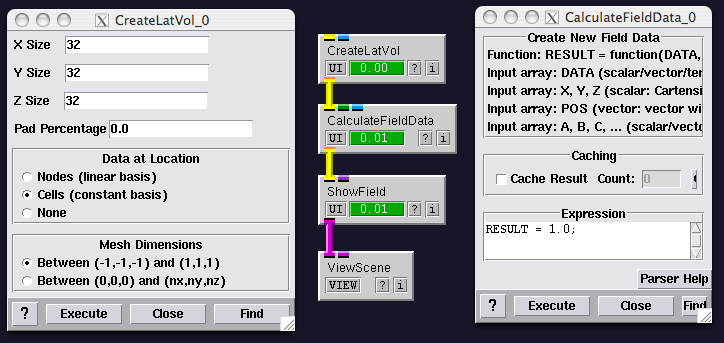
\includegraphics{DefibrillationTutorial_figures/network_1.png}}
\caption{Network to generate hexahedral
mesh.}\label{fig:hexMeshNetwork}
\end{figure}

Open the user interface to the {\bf CreateLatVol} module and specify
the number of nodes to be 32x32x32 by typing those values into the ``X
Size'', ``Y Size'', and ``Z Size'' fields. We will be solving this
problem with data located in the cells, rather than at the nodes, so
chose ``Cells (constant basis)'' in the ``Data at Location'' panel.
Open the user interface to
the {\bf CalculateFieldData} module, and set the expression to {\tt
RESULT~=~1.0;} to set the entire field to a value of 1.0. Click the
``Execute All'' button to run the networks and click the ``VIEW''
button on the {\bf ViewScene} module to view the results. You should
see something similar to the results shown in Figure
\ref{fig:step_1_results}. The images shown in this tutorial may not be
the default rendering view. Manual rotation using the center mouse
button may be required for your image to match those here.

\begin{figure}
\scalebox{0.3}{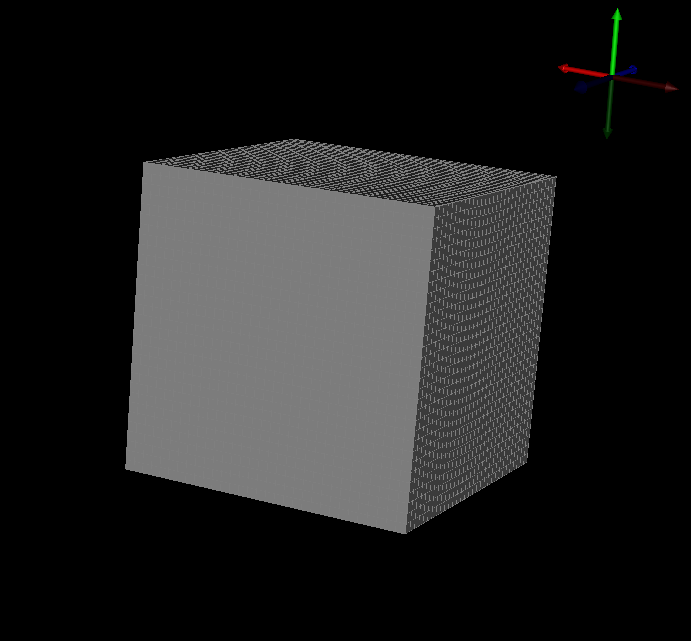
\includegraphics{DefibrillationTutorial_figures/step_1_result.png}}
\caption{Generated hexahedral mesh}\label{fig:step_1_results}
\end{figure}

\section{Creating Plate Electrode Geometry}

The next step in building our network is to add plate anodes and
cathodes to the simulation. The electrodes will be modeled as boxes,
but this time we will use {\bf EditMeshBoundingBox} modules to allow
the user to resize and reposition the electrodes interactively.  Add
another {\bf CreateLatVol} to the network, this time setting the ``X Size'', ``Y Size'', and ``Z Size'' fields to {\tt 2}.
Connect this new module to two separate {\bf
EditMeshBoundingBox} modules, one for the anode and one for the
cathode. The {\bf EditMeshBoundingBox} module will output a new
transformed field and an editable visualization widget. Connect the
yellow field output ports to {\bf ShowField} modules, and connect the
pink output ports of both {\bf EditMeshBoundingBox} modules and the
new {\bf ShowField} modules to the {\bf ViewScene} module. The
modified network should look like that in Figure \ref{fig:network_2}.

\begin{figure}
\scalebox{0.5}{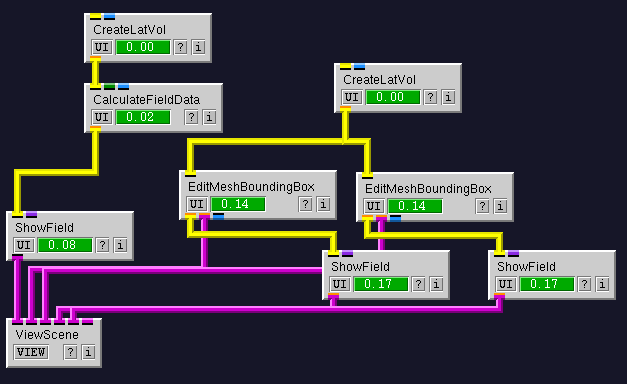
\includegraphics{DefibrillationTutorial_figures/network_2.png}}
\caption{Adding plate electrodes to the network.}\label{fig:network_2}
\end{figure}

Before viewing this new network, we want to edit the new {\bf
ShowField} modules to distinguish the two electrodes. Open the first
{\bf ShowField} module, click on the ``Faces'' tab, and check the
``Enable Transparency'' checkbox. Click on the ``Default Color''
button, and change the color by adding red. Performing these same
operations on the second {\bf ShowField} module, this time adding more
green to the color. These operations are shown in Figure
\ref{fig:network_2_show_field}.

\begin{figure}
\scalebox{0.4}{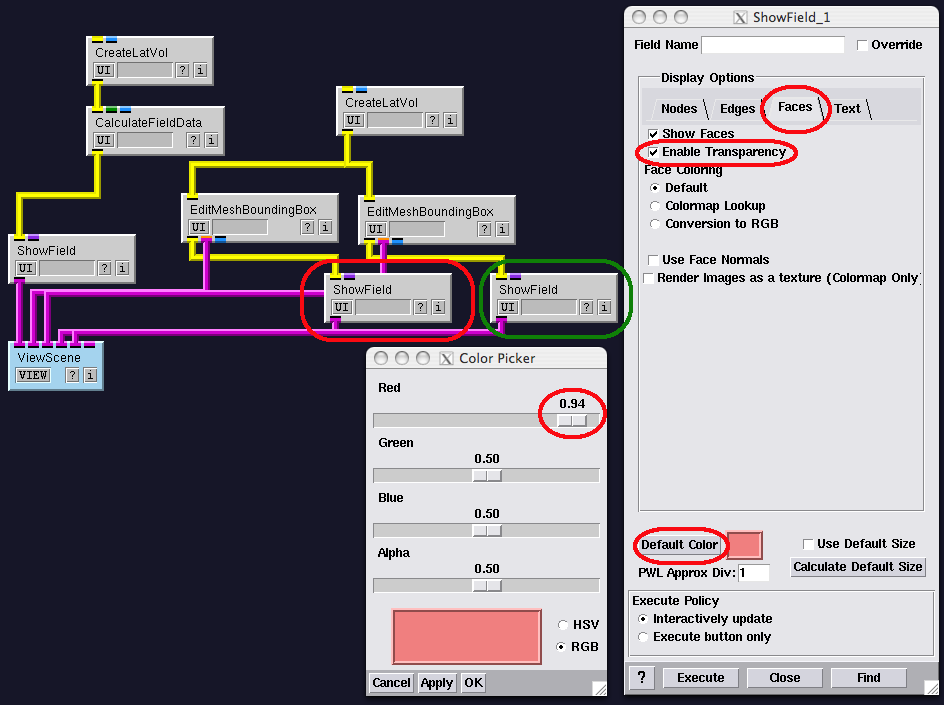
\includegraphics{DefibrillationTutorial_figures/network_2_show_field.png}}
\caption{Editing the {\bf ShowField} modules for the
electrodes.}\label{fig:network_2_show_field}
\end{figure}

The network can now be viewed and the positions of the electrodes can
be modified in the view window by holding down the Shift key and using
the left mouse button to either grab the borders of the electrodes
(shown as grey lines) and moving the box, or grab the small cylinders
on the box faces and resizing the box. Alternatively, the position and
sizes of the electrodes can be set manually in the {\bf
EditMeshBoundingBox} modules.

To manually set the electrode size, open the user interface to the
first {\bf EditMeshBoundingBox}, make sure the ``Center'' and ``Size''
check boxes are checked, and enter values for the center position and
size. The remainder of this tutorial will use center and size values
of (-1.0,~0.5,~0.5) and (0.2,~1.5,~1.5) for the first electrode and
(1.0,~-0.5,~-0.5) and (0.2,~1.5,~1.5) for the second electrode. An
example of this operation is shown in Figure
\ref{fig:network_2_edit_mesh}.

\begin{figure}
\scalebox{0.5}{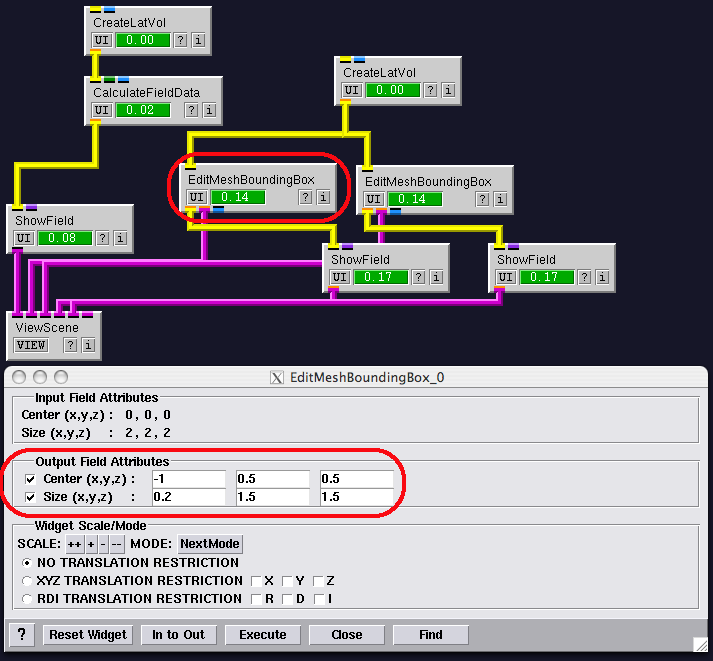
\includegraphics{DefibrillationTutorial_figures/network_2_edit_mesh.png}}
\caption{Editing the {\bf EditMeshBoundingBox} modules for the
electrodes.}\label{fig:network_2_edit_mesh}
\end{figure}

Finally, we can view the scene with all our required geometry, by
clicking the ``Execute All'' button and clicking ``VIEW'' on the {\bf
ViewScene} module. Results should be similar to those in Figure
\ref{fig:step_2_results}.

\begin{figure}
\scalebox{0.3}{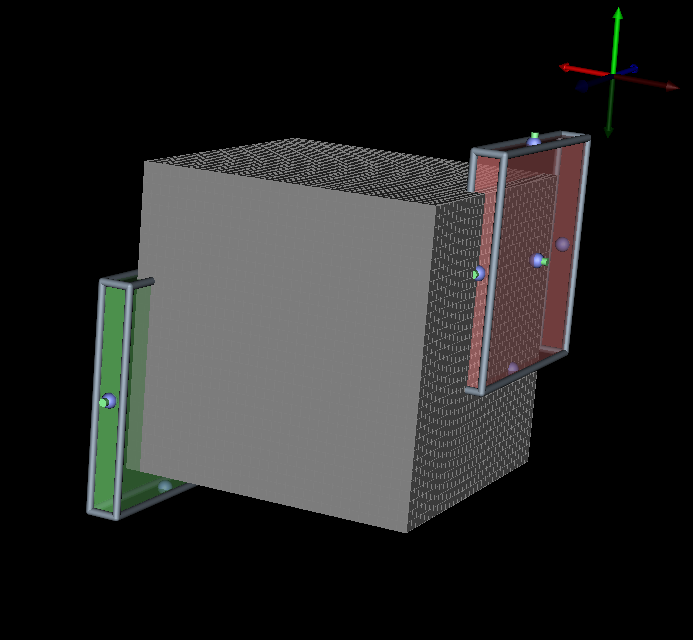
\includegraphics{DefibrillationTutorial_figures/step_2_results.png}}
\caption{Geometry for the problem, including a box simulation domain
and two electrodes (red and green).}\label{fig:step_2_results}
\end{figure}

\section{Building and Solving the Finite Element Simulation}

Now that we have the geometry for our problem defined, we need to
build our finite element matrices, set our known values, and solve the
simulation. To begin, connect a {\bf CalculateFieldData} module
between each of the {\bf EditMeshBoundingBox} modules and their
respective {\bf ShowField} modules. Open the first {\bf
CalculateFieldData} module and set the expression to {\tt
RESULT~=~0;}. The expression in the second {\bf CalculatFieldData}
module should be set to {\tt RESULT~=~700;}. These are the known
electric potentials assigned to the two electrodes. The resulting
network is shown in Figure \ref{fig:network_3_calc_field_data}.

\begin{figure}
\scalebox{0.4}{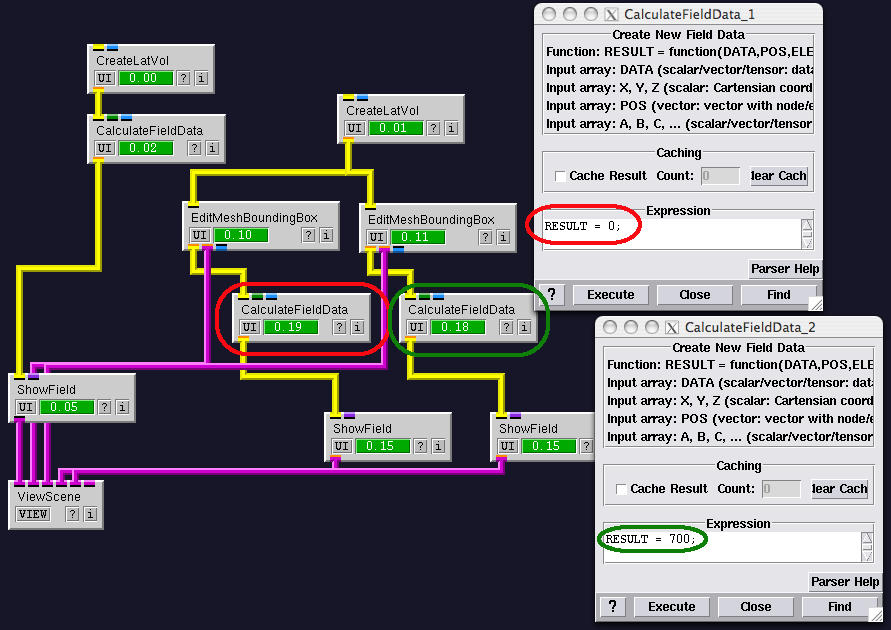
\includegraphics{DefibrillationTutorial_figures/network_3_calc_field_data.png}}
\caption{Setting potentials for the
electrodes.}\label{fig:network_3_calc_field_data}
\end{figure}

Next, we want to map the assigned potentials as known values onto
corresponding nodes of the hexahedral mesh. This is accomplished by
first joining the two electrode fields together using the {\bf
JoinFields} module, connecting the yellow outputs of the electrodes'
{\bf CalculateFieldData} modules to the first two inputs on the {\bf
JoinFields} module. Next, these values are mapped onto nodes in the
Hex mesh using the {\bf MapFieldDataOntoNodes} module. The output of
the {\bf JoinFields} module is connected to the first input of the
{\bf MapFieldDataOntoNodes} module while the output of the {\bf
CalculateFieldData} of the Hex mesh is connected to the third input.

The linear system solver in SCIRun uses values of NaN (not a number)
to specify unknowns in one of the input vectors, and our added {\bf
MapFieldDataOntoNodes} module will also be used to set values in the
mesh outside of the electrodes to NaN. To do this, open the user
interface for the module and set the ``Default Outside Value'' to {\tt
nan} and the ``Maximum Distance'' to {\tt inf}.

The values on the nodes now represent both the unknown (NaN) and known
values of our system. We our now ready to build our finite element
linear system. To do so, add a {\bf BuildFEMatrix} module into the
network, connecting the output of the Hex mesh {\bf
CalculateFieldData} module to the input of the {\bf BuildFEMatrix}
module. To specify the known values, first connect the output of the
{\bf MapFieldDataOntoNodes} to a {\bf GetFieldData} module. Next, add
a {\bf AddKnownsToLinearSystem} module to the network, connecting the
{\bf BuildFEMatrx} to the first input, and the output of the {\bf
GetFieldData} to the third input. The current state of the network
should look like Figure \ref{fig:network_4_map_field_data}.

\begin{figure}
\scalebox{0.4}{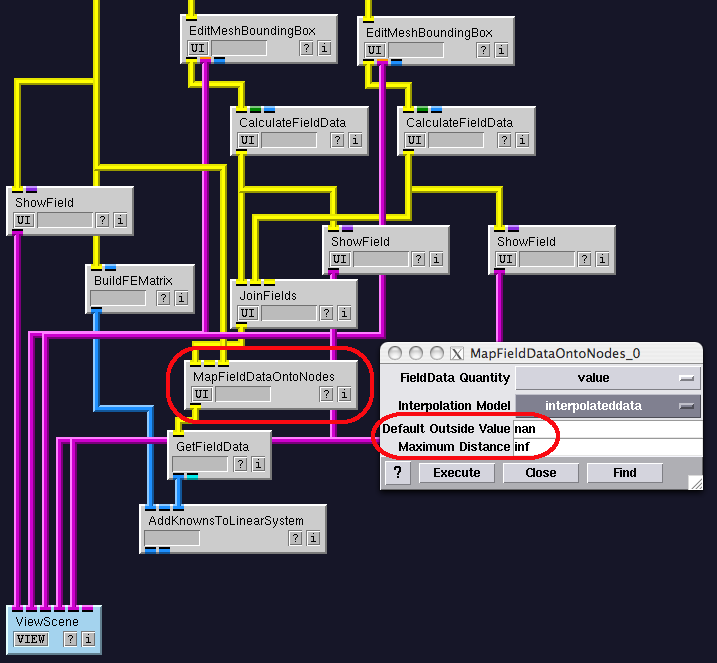
\includegraphics{DefibrillationTutorial_figures/network_4_map_field_data.png}}
\caption{Network after adding {\bf AddKnownsToLinearSystem}
module.}\label{fig:network_4_map_field_data}
\end{figure}

Continuing, we will solve the linear system, connecting the two
outputs of the {\bf AddKnownsToLinearSystem} to the two inputs of a
new {\bf SolveLinearSystem} module. The first output of the solver
will contain the solution values. We map this onto the mesh by adding
a {\bf SetFieldData} module, connecting the outputs of the {\bf
MapFieldDataOntoNodes} and {\bf SolveLinearSystem} modules to the
first two inputs of the {\bf SetFieldData} module. To visualize the
field, we connect the output of the {\bf SetFieldData} into a new {\bf
ShowField} module and connect that {\bf ShowField} module to our {\bf
ViewScene} module. To make the visualization useful, we will create a
color map by adding a {\bf CreateStandardColorMaps} and connecting the
output to a {\bf RescaleColorMap} module. The output of the {\bf
SetFieldData} module is used as the second input to the {\bf
RescaleColorMap} module. And lastly, the output of the {\bf
RescaleColorMap} module is used as the second input to the last {\bf
ShowField} module. We now have a color mapped version of our Hex mesh
as an input to the {\bf ViewScene} module, so be sure to delete the
original input to the {\bf ViewScene} module coming from the Hex mesh
visualization. The final piece of the network is shown in
Figure~\ref{fig:network_5} and the expected output is shown in
Figure~\ref{fig:step_5_results_pre_vis_settings}.

\begin{figure}
\scalebox{0.4}{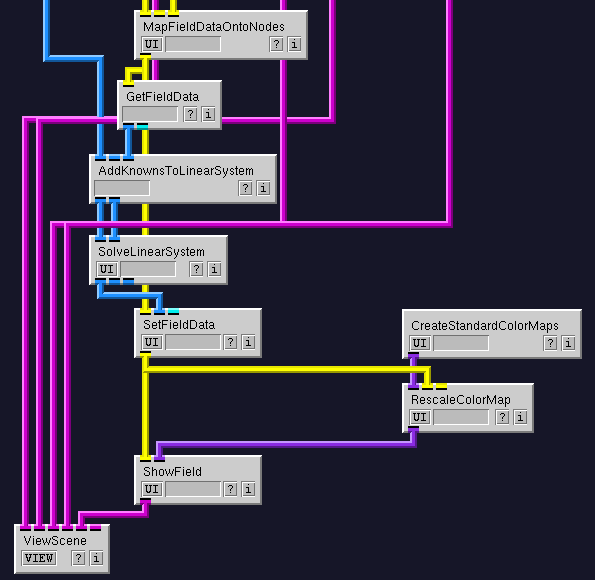
\includegraphics{DefibrillationTutorial_figures/network_5.png}}
\caption{Final simulation network for the two electrode
problem.}\label{fig:network_5}
\end{figure}

\begin{figure}
\scalebox{0.3}{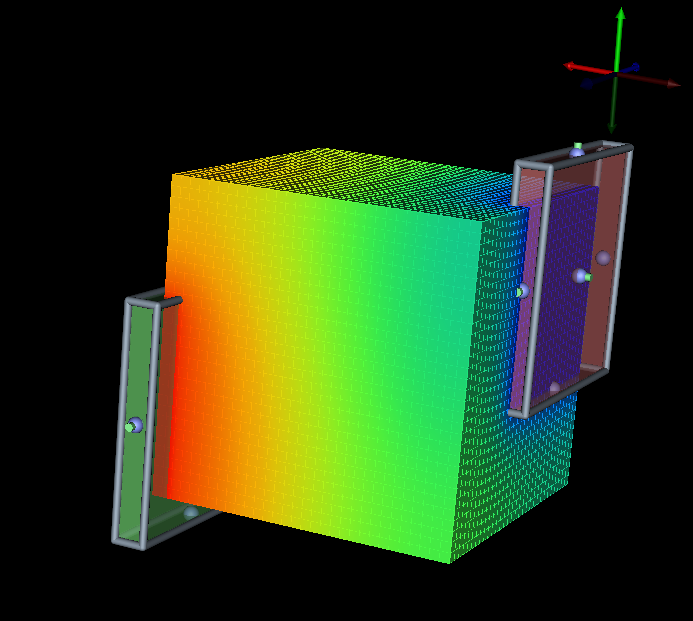
\includegraphics{DefibrillationTutorial_figures/step_5_results_pre_vis_settings.png}}
\caption{Results of the finite element simulation with two
electrodes.}\label{fig:step_5_results_pre_vis_settings}
\end{figure}

Lastly, the visualization can be made more appealing by making a few
changes to the {\bf CreateStandardColorMaps} module and the last {\bf
ShowField} module. First, open the user interface to the last {\bf
ShowField} module and uncheck the ``Show Nodes'' and ``Show Edges''
boxes on the ``Nodes'' and ``Edges'' tabs. This will result in a
visualization only showing faces with a smooth gradient. Another
effective change is to force the color map to have less resolution.
Open the {\bf CreateStandardColorMaps} user interface and change the
``Resolution'' slider to a setting of 25. This will result in a less
smooth color mapping, where the boundaries of the discrete colors act
as contour lines of the solution on the surface of the domain. These
user interface changes are shown in
Figure~\ref{fig:network_5_view_settings} and the new output is shown
in Figure~\ref{fig:step_5_results}.

\begin{figure}
\scalebox{0.4}{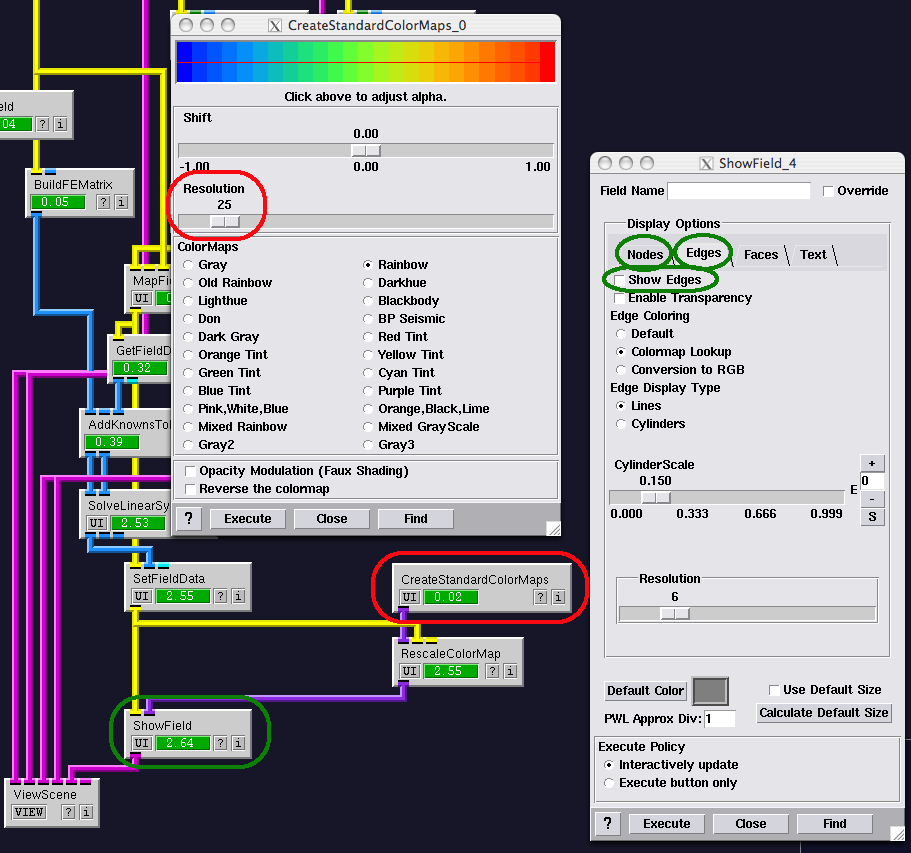
\includegraphics{DefibrillationTutorial_figures/network_5_view_settings.png}}
\caption{Changing the {\bf ShowField} and {\bf
CreateStandardColorMaps} settings for an effective
visualization.}\label{fig:network_5_view_settings}
\end{figure}

\begin{figure}
\scalebox{0.3}{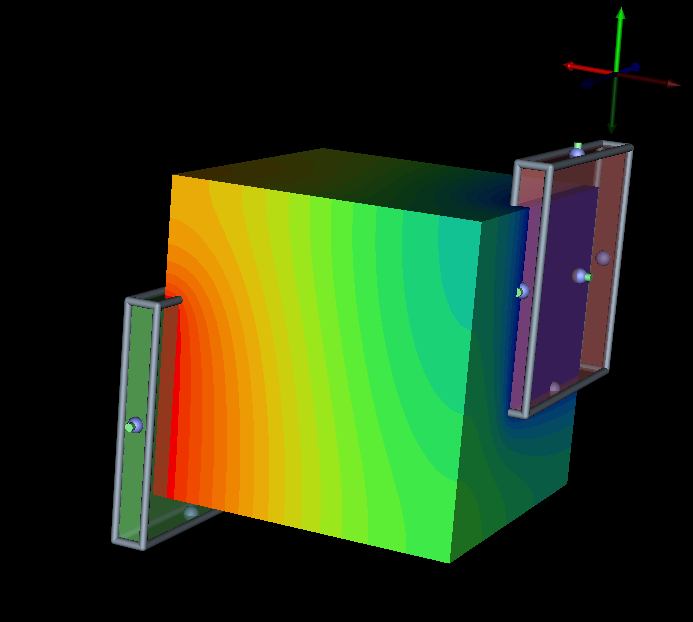
\includegraphics{DefibrillationTutorial_figures/step_5_results.png}}
\caption{Results of the finite element simulation with two electrodes
after adjusting view settings.}\label{fig:step_5_results}
\end{figure}

As a reminder, the positions and sizes of the electrodes in the
visualization are interactively editable. The electrodes can be moved
and the simulation will be rerun with the new electrode geometry.

\section{Adding a Floating Lead}

Of interest to some, is the addition of a floating lead into the
simulation, {\em i.e.} an extra conductor without a known potential.
The procedure for doing so begins with adding a third {\bf
EditMeshBoundingBox} module connected to a {\bf ShowField} module,
changing the {\bf ShowField} settings to enable transparency and
setting the default color this time to something blue. Connect the
pink outputs of both the {\bf EditMeshBoundingBox} and {\bf
ShowField} modules to the {\bf ViewScene} module. In the remainder of
this tutorial, the third {\bf EditMeshBoundingBox} was set to have a
center value of (0.3,~0.5,~-0.5) and a size of (0.5,~1.2,~1.2) in the
user interface. The modified network is shown in
Figure~\ref{fig:network_6_a_add_blue_blox} and the resulting
visualization is shown in Figure~\ref{fig:step_6_a_results}. Note that
the addition of this geometry has not affected the solution.

\begin{figure}
\scalebox{0.4}{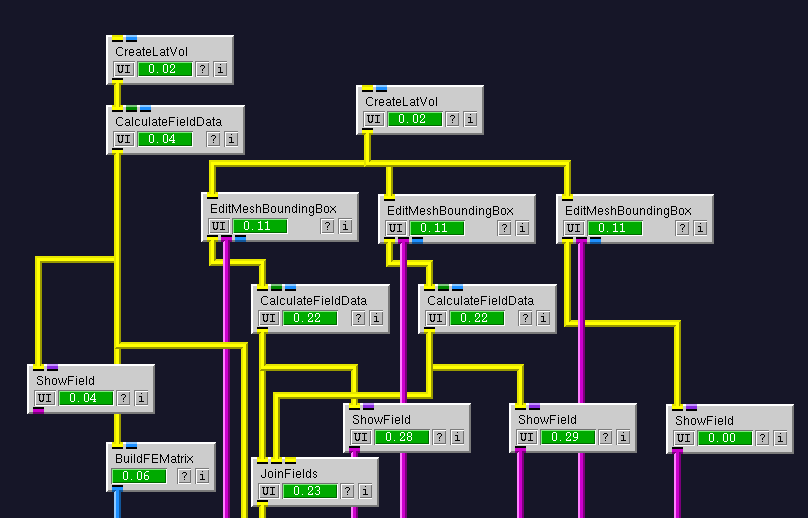
\includegraphics{DefibrillationTutorial_figures/network_6_a_add_blue_blox.png}}
\caption{Adding a floating lead to the problem
geometry.}\label{fig:network_6_a_add_blue_blox}
\end{figure}

\begin{figure}
\scalebox{0.3}{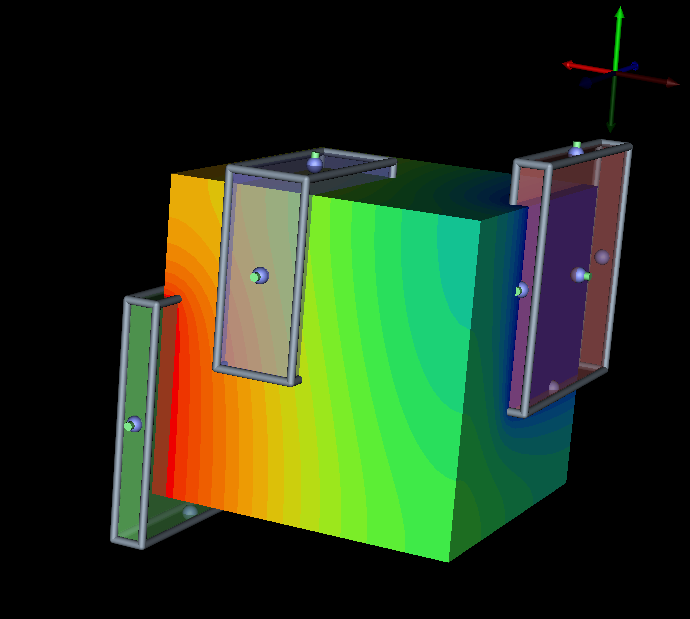
\includegraphics{DefibrillationTutorial_figures/step_6_a_results.png}}
\caption{Simulation with added floating lead
geometry.}\label{fig:step_6_a_results}
\end{figure}

Next, we need to know which of the nodes are inside this new
conductor. To calculate this, add a {\bf CalculateInsideWhichField}
module to the network, with the first input coming from the first hex
mesh {\bf CalculateFieldData} output, and the second input coming from
the third {\bf EditMeshBoundingBox} output. We again want nodes
outside of the new conductor to be set to NaN, and values inside set
to 1.0. Open the user interface and set the ``Default outside value''
to {\tt nan}, the ``Value assigned to first field'' to {\tt 1.0}, the
``Datatype of destination field'' to {\tt float} and the ``Output data
location'' to {\tt node}. The addition of this module and the user
interface settings are shown in Figure
\ref{fig:network_6_calculateInside}.

\begin{figure}
\scalebox{0.4}{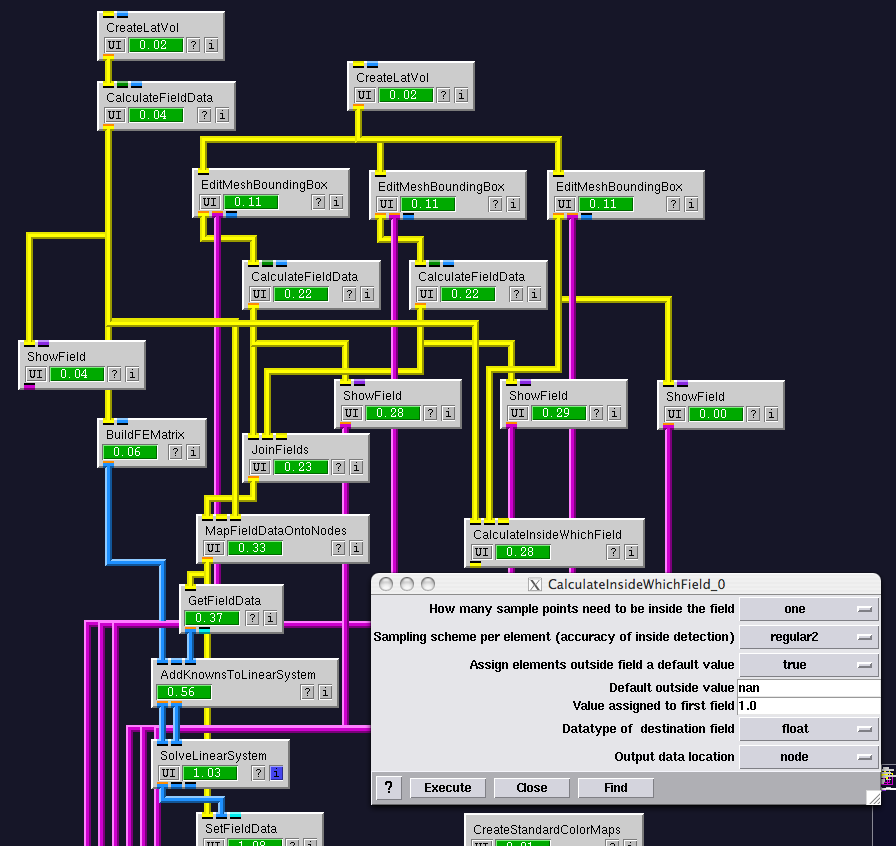
\includegraphics{DefibrillationTutorial_figures/network_6_calculateInside.png}}
\caption{Network and user interface settings when adding the {\bf
CalculateInsideWhichField}
module.}\label{fig:network_6_calculateInside}
\end{figure}

The effect of adding a conductor into the problem domain is that the
solution will be constant for all nodes inside the conductor. For this
to happen, we need to modify the linear system and ``link'' all the
nodes inside the conductor to have the same solution value. To do
this, connect a {\bf GetFieldData} module to the output of the {\bf
CalculateInsideWhichField} module. Next, delete the connections
between {\bf AddKnownsToLinearSystem} and {\bf SolveLinearSystem} and
add a {\bf AddLinkedNodesToLinearSystem} module between these two,
connecting the first two outputs of {\bf AddKnownsToLinearSystem} to
the first two inputs of {\bf AddLinkedNodesToLinearSystem}. Connect
{\bf AddLinkedNodesToLinearSystem} and {\bf SolveLinearSystem} in the
same way. The third input for the {\bf AddLinkedNodesToLinearSystem}
module comes from the output of the new {\bf GetFieldData} module.
Next, add an {\bf EvaluateLinAlgBinary} module with the first input
coming from the third output of the {\bf AddLinkedNodesToLinearSystem}
module. Delete the output of {\bf SolveLinearSystem} and connect it
instead to the second input of {\bf EvaluateLinAlgBinary}. The output
from {\bf EvaluateLinAlgBinary} is now the second input for {\bf
SetFieldData}. This completes the modifications to the simulation. The
final modified network is shown in Figure \ref{fig:network_6_b} and
the simulation results are shown in Figure \ref{fig:step_6_results}.

\begin{figure}
\scalebox{0.4}{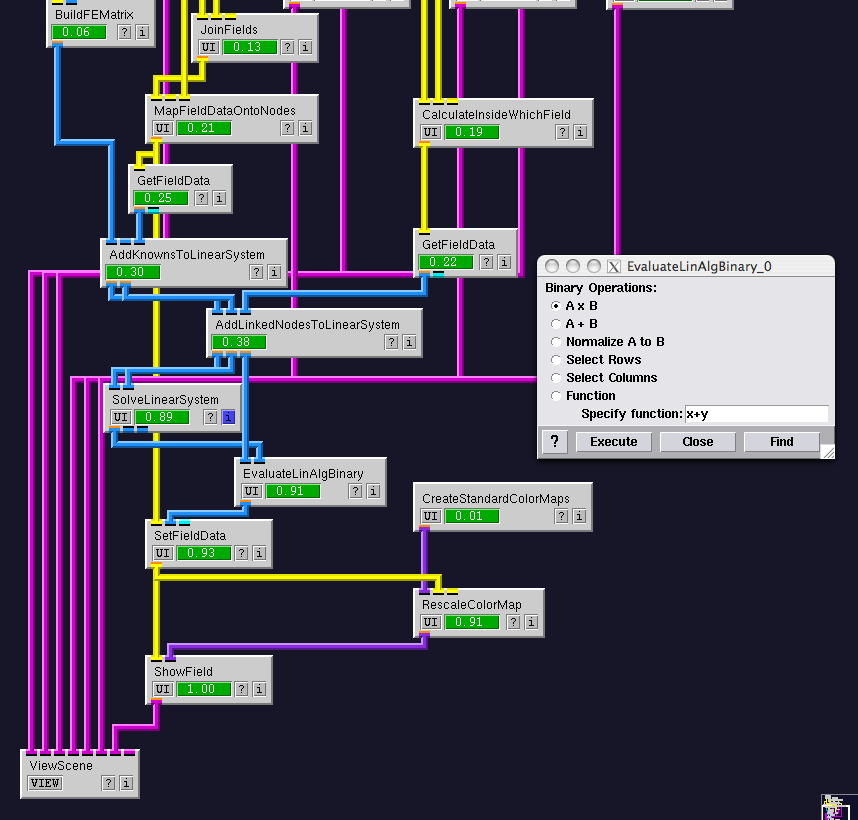
\includegraphics{DefibrillationTutorial_figures/network_6_b.png}}
\caption{Completing the network with an added floating
lead.}\label{fig:network_6_b}
\end{figure}

\begin{figure}
\scalebox{0.3}{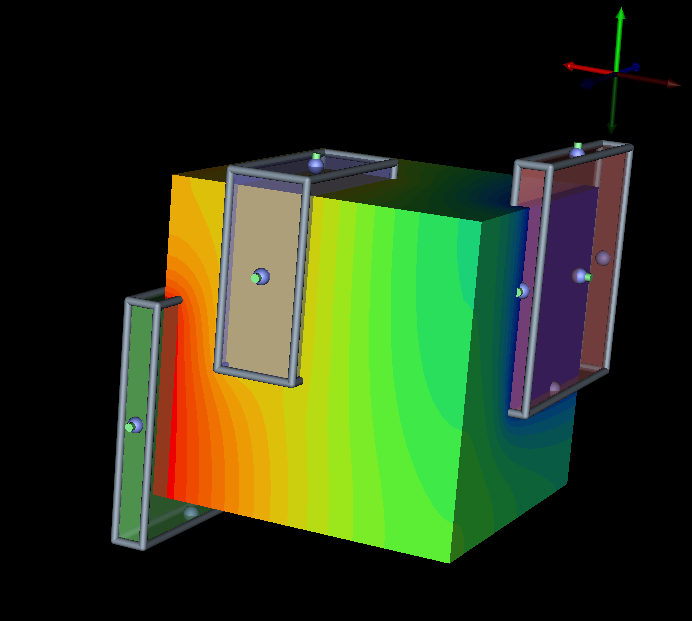
\includegraphics{DefibrillationTutorial_figures/step_6_results.png}}
\caption{Simulation results with an added floating
lead.}\label{fig:step_6_results}
\end{figure}

The fact that the solution field is constant inside the floating lead
is difficult to see when the floating lead is visible. Figure
\ref{fig:step_6_results_noface} shows a final visualization where the
``Show Faces'' checkbox inside of the {\bf ShowField} module
corresponding the the floating lead is unchecked. Now, the constant
field is easy to discern.

\begin{figure}
\scalebox{0.3}{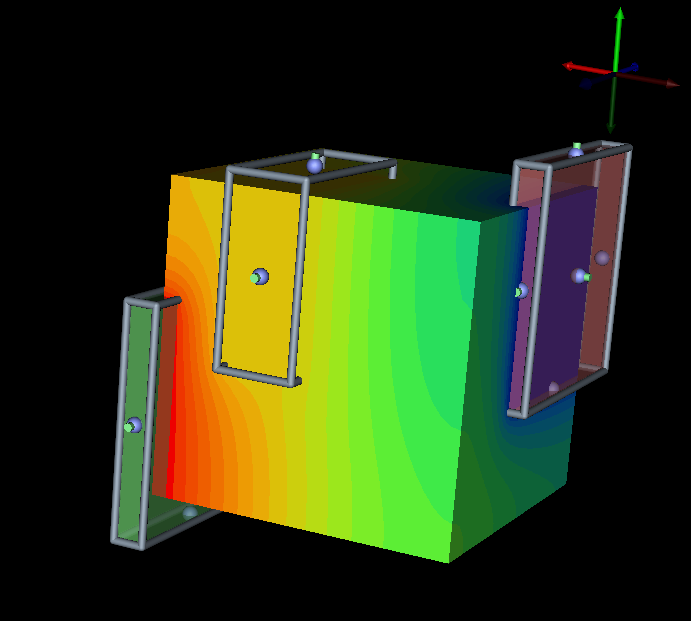
\includegraphics{DefibrillationTutorial_figures/step_6_results_noface.png}}
\caption{Simulation results with an added floating lead with the
visualization of the floating lead's faces turned
off.}\label{fig:step_6_results_noface}
\end{figure}

\chapter{Placing Electrodes}

In the previous chapter, we learned how to run a finite element
simulation on a cube with two electrodes and a floating lead. In the
remaining sections, we will perform a similar calculation on a human
torso using previously segmented torso data, a model of a can
electrode, a wire electrode, and a planar electrode.

\section{Loading The Dataset}\label{sec:loading}

Start SCIRun and insert a {\bf ReadField} module into the
network. Open the user interface, select ``SCIRun Field File (*.fld)''
from the ``Files of type'' drop-down menu, browse to and select the
{\tt torso-defib/torso\_segmentation\_si.fld} file. Unlike the cube above, we are
interested in the internal structure of this file, so we will use
texture slices to view the data.

Connect the output of {\bf ReadField} to a {\bf
ConvertFieldsToTexture} module and connect that module to a {\bf
ShowTextureSlices} module. Open the user interface to {\bf
ShowTextureSlices} and check the ``X plane'', ``Y plane'', and ``Z
plane'' boxes. Place a {\bf CreateStandardColorMaps} module in the
network, and connect its output to the second input of the {\bf
ShowTextureSlices} module. Open the {\bf CreateStandardColorMaps} user
interface and click the mouse in the upper display to adjust
alpha. Create one point in the lower left corner (this will make the
area outside the torso black). Create another point back near the
middle of the display, slightly to the right of the first
point. Finally, connect the {\bf ShowTextureSlices} output to a new
{\bf ViewScene} module. The network should look similar to that shown
in Figure \ref{fig:p_e_network_1} and the display output is shown in
Figure \ref{fig:p_e_results_1}.
 
\begin{figure}
\scalebox{0.4}{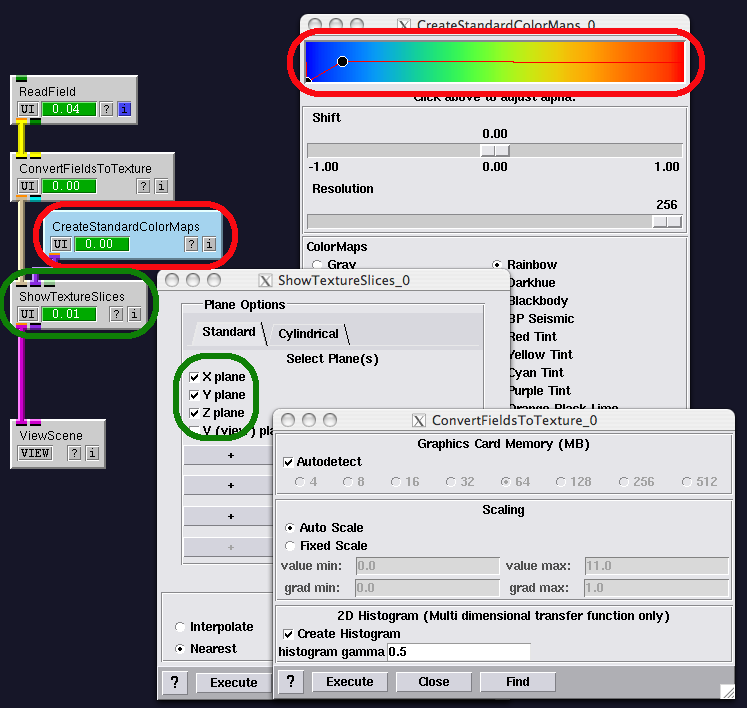
\includegraphics{DefibrillationTutorial_figures/place_electrodes_network_1.png}}
\caption{Start of a network to place electrodes in
torso.}\label{fig:p_e_network_1}
\end{figure}

\begin{figure}
\scalebox{0.3}{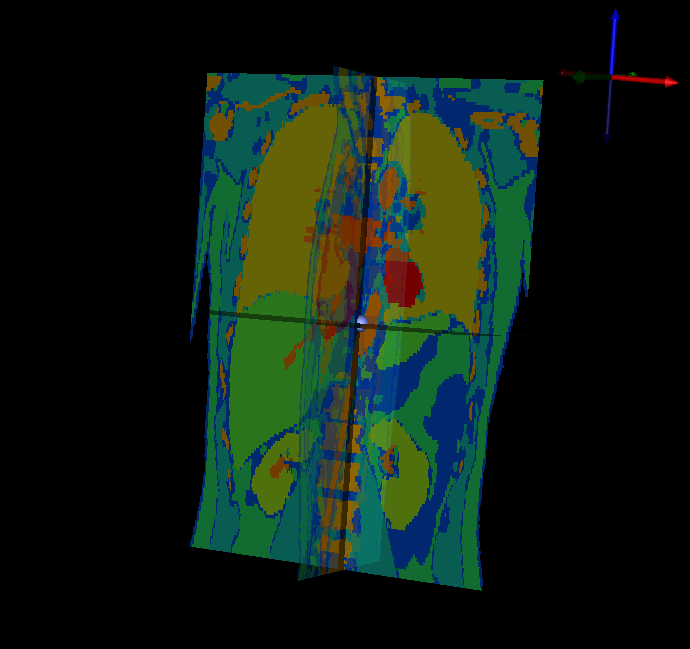
\includegraphics{DefibrillationTutorial_figures/place_electrodes_results_1}}
\caption{Output of initial torso
visualization.}\label{fig:p_e_results_1}
\end{figure}

\section{Visualizing Extra Geometry}

The visualization in Section \ref{sec:loading} shows texture slices
through the entire segmented torso. One may also be interested in
adding additional 3D visualizations of subsets of the segmentation to
aid in the placement of electrodes. Next, we will add a visualization
of the boundary of the heart as an example.

Add the following module chain to the network: Connect the {\bf
ReadField} module to a {\bf GetDomainBoundary} module, followed by a
{\bf FairMesh} module, and lastly a {\bf ShowField} module. The output
of {\bf ShowField} should be connected as the second input to the {\bf
ViewScene} module.

Open the user interface to the {\bf GetDomainBoundary} module, make
sure the ``Only include compartments in the range between'' checkbox
is checked, and put values of {\tt 10} and {\tt 11} for the ``min:''
and ``max:'' fields. Also, make sure ``Include outer boundary'' is
checked. Next, open the user interface to the {\bf ShowField}
module. As before, Disable the viewing of the nodes and edges, and
enable transparency for the faces. Set the ``Face Coloring'' to
``Default'' and select a red default color. The new network should
look like Figure \ref{fig:p_e_network_2} and the resulting
visualization is shown in \ref{fig:p_e_results_2}.

\begin{figure}
\scalebox{0.4}{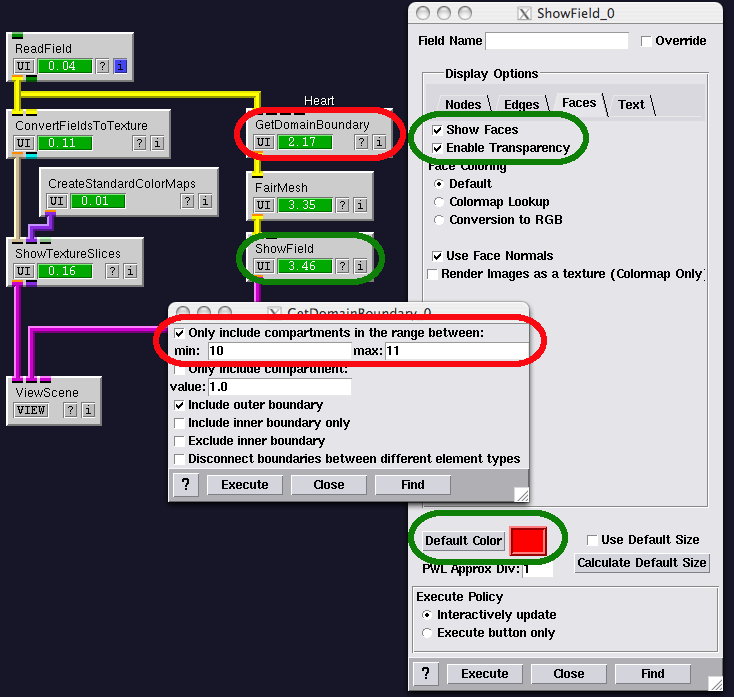
\includegraphics{DefibrillationTutorial_figures/place_electrodes_network_2.png}}
\caption{Network after adding visualization of the
heart.}\label{fig:p_e_network_2}
\end{figure}

\begin{figure}
\scalebox{0.3}{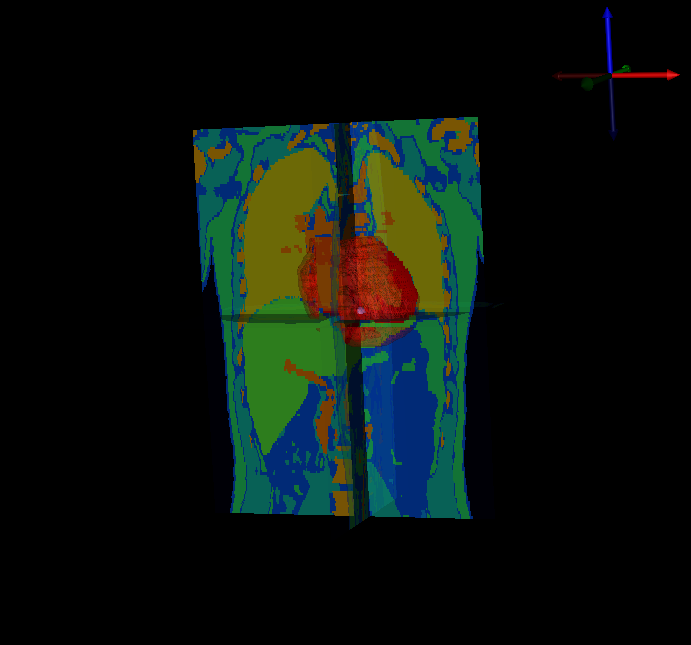
\includegraphics{DefibrillationTutorial_figures/place_electrodes_results_2}}
\caption{Visualization results, including
heart.}\label{fig:p_e_results_2}
\end{figure}

Next, a visualization of the outer boundary of the dataset may be
useful. Add a similar module chain as for the heart, but this time in
the new {\bf GetDomainBoundary} module, only include compartments in
the range between {\tt 1} and {\tt 255}. This will select all
data. Also, we are only interested in the outer boundary of this data
set, so make sure both ``Include outer boundary'' and ``Exclude inner
boundary'' are both checked. The network and results are shown in
Figures \ref{fig:p_e_network_3} and \ref{fig:p_e_results_3}.

\begin{figure}
\scalebox{0.4}{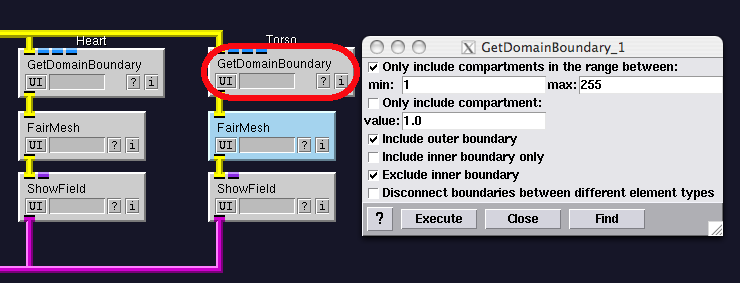
\includegraphics{DefibrillationTutorial_figures/place_electrodes_network_3.png}}
\caption{Addition of outer torso boundary visualization to the
network.}\label{fig:p_e_network_3}
\end{figure}

\begin{figure}
\scalebox{0.3}{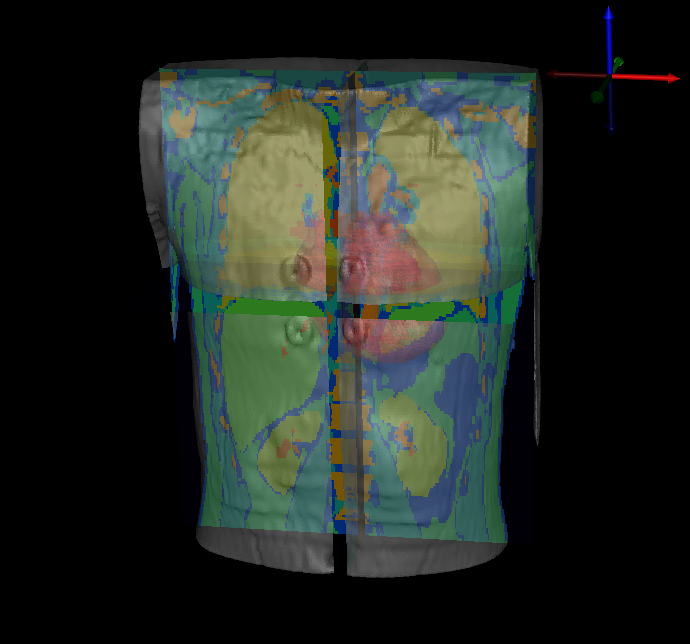
\includegraphics{DefibrillationTutorial_figures/place_electrodes_results_3}}
\caption{Visualization results, including heart and
torso.}\label{fig:p_e_results_3}
\end{figure}

Other subsets of the segmentation can also be added to the
visualization. Table \ref{tbl:seg_values} lists the segmentation
indices in the torso dataset.

\begin{table}
\begin{tabular}{|l|l|}
\hline
{\bf Material} & {\bf Seg. Indx}\\ \hline
\hline
Background & 0\\ \hline
Connective Tissue & 1\\ \hline
Bowel Gas & 2 \\ \hline
Muscle & 3 \\ \hline
Fat & 4 \\ \hline
Kidney & 5 \\ \hline
Liver & 6 \\ \hline
Lung & 7 \\ \hline
Bone & 8 \\ \hline
Blood & 9 \\ \hline
Heart-Atria & 10 \\ \hline
Heart-Ventricles & 11 \\ \hline
\end{tabular}
\caption{Table of segmentation indices in the torso dataset.}
\label{tbl:seg_values}
\end{table}

\section{Adding a Can Electrode}

Next, we will read in a model of a can electrode and send the model
through a widget that will allow interactive editing of the
electrodes' placement and size. Begin by adding another {\bf
ReadField} module to the network. Open the user interface, select
``SCIRun Field File (*.fld)'' from the ``Files of type'' drop-down
menu, browse to and select the {\tt torso-defib/electrode\_can\_model\_si.fld}
file. Connect the output of {\bf ReadField} to an {\bf
EditMeshBoundingBox} module. Connect the pink output of {\bf
EditMeshBoundingBox} directly to the {\bf ViewScene} module - this
will allow the visualization of the widget. Connect the yellow output
to a new {\bf ShowField} which is also connected to {\bf
ViewScene}. Open the {\bf ShowField} user interface, disable the
viewing of nodes and edges, and select the default color to be
something green.

Similar to the placing of electrodes in the cube mesh previously, upon
viewing the scene the location and size of the electrode can be
modified through interaction with the {\bf EditMeshBoundingBox}
widget. Holding the shift key and grabbing the various controls
(edges, spheres, and cylinders) will modify the position, rotation,
and scaling of the electrode. Figure \ref{fig:p_e_network_4} shows
this modified network and Figure \ref{fig:p_e_results_4} shows the
placement used in the remainder of this tutorial.

\begin{figure}
\scalebox{0.4}{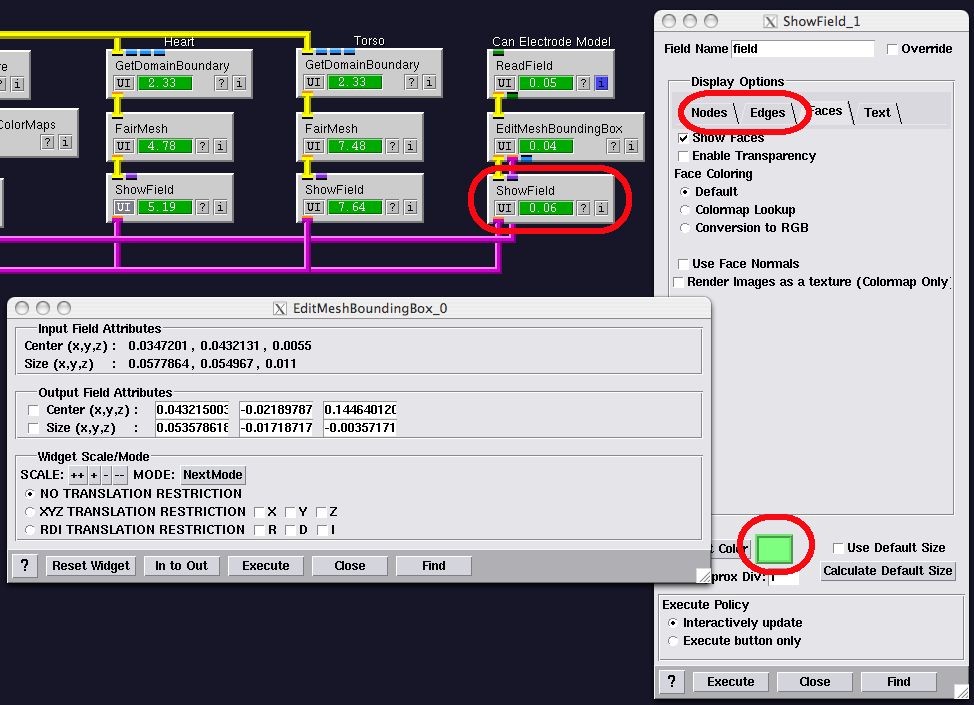
\includegraphics{DefibrillationTutorial_figures/place_electrodes_network_4.png}}
\caption{Addition of a can electrode to the
network.}\label{fig:p_e_network_4}
\end{figure}

\begin{figure}
\scalebox{0.3}{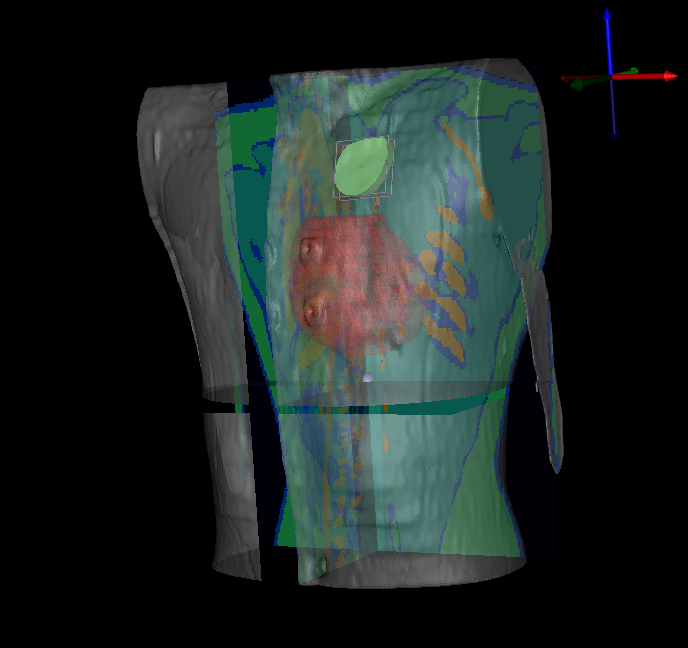
\includegraphics{DefibrillationTutorial_figures/place_electrodes_results_4}}
\caption{Placement of the can electrode.}\label{fig:p_e_results_4}
\end{figure}

\section{Adding a Wire Electrode}

A second type of electrode often used in defibrillation scenarios is a
wire. In this section, we will create a small cylinder which
represents the non-insulated section of a wire electrode lead. SCIRun
provides a widget to generate and manipulate a wire electrode. Add a
{\bf GenerateElectrode} module to the network, connecting the
pink output port to the {\bf ViewScene} module and the yellow output
port to a new {\bf ShowField} module. Again, connect the {\bf
ShowField} module to the {\bf ViewScene} module. Open the {\bf
GenerateElectrode} module and to start, set the length of the
electrode to {\tt 0.1} (corresponding to 10 centimeters). Set the
width of the electrode to {\tt 0.003}. Open the {\bf ShowField}
module, turn off visualization of the nodes and edges, and set the
default color to something distinctive. Figure \ref{fig:p_e_network_4}
shows an example of this modified network.

\begin{figure}
\scalebox{0.4}{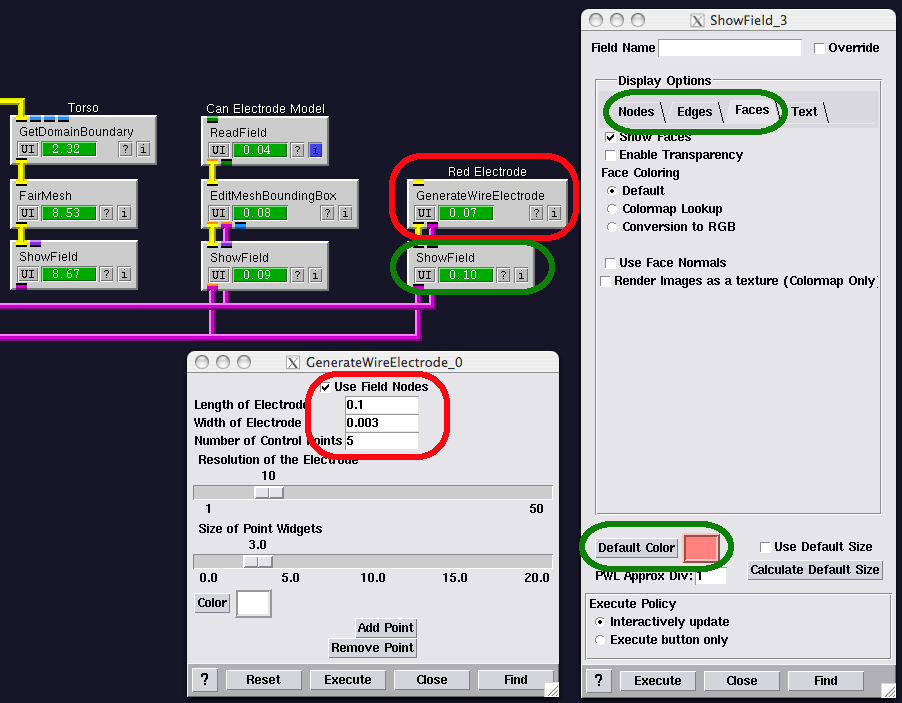
\includegraphics{DefibrillationTutorial_figures/place_electrodes_network_5.png}}
\caption{Addition of a wire electrode.}\label{fig:p_e_network_5}
\end{figure}

Upon viewing the scene, a wire electrode will now be present. On the
wire electrode, 5 control points will be visible. Moving the control
points changes the shape of the electrode in a fairly intuitive
manner. Note that the electrode does not necessarily travel through
the points, they are only used as control points for a spline
function. Also note that the electrode will always start at one of the
points, but will not necessarily end at the last point. The length is
determined by the length value in the user interface, not the position
of the last point. Figure \ref{fig:p_e_results_5} shows an example of
the electrode placement used in the remainder of this tutorial.

\begin{figure}
\scalebox{0.3}{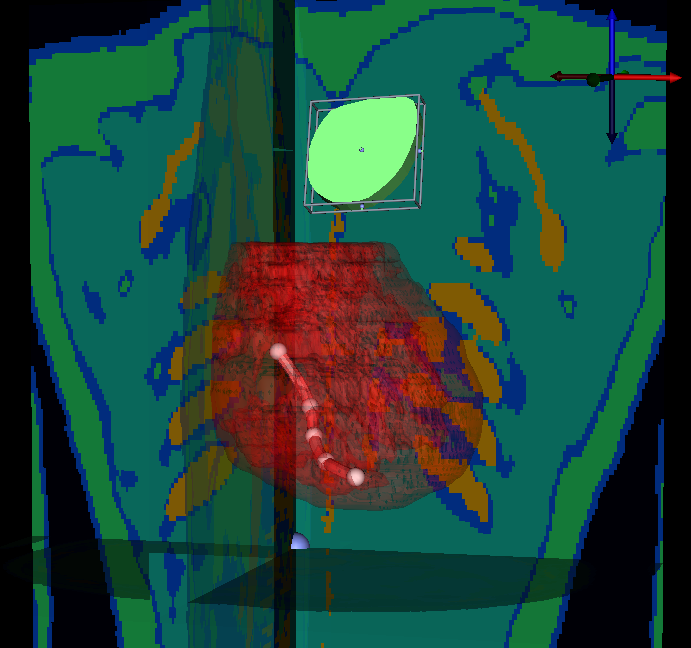
\includegraphics{DefibrillationTutorial_figures/place_electrodes_results_5}}
\caption{Placement of the wire electrode.}\label{fig:p_e_results_5}
\end{figure}

\section{Adding a Planar Electrode}

Lastly, we will add a planar electrode. The creation of the planar
electrode is similar to the wire electrode, with the exception that
the planar electrode has a length, width, thickness, and normal vector
rather than just a length and width. Similar to the wire electrode,
add a {\bf GenerateElectrode} module, connected to a {\bf
ShowField} module, both connected to the {\bf ViewScene} module. Open
the {\bf GenerateElectrode} user interface, select the "Planar Electrode" radio button, set the length of
the electrode to {\tt 0.1}, thickness to {\tt 0.003}, and width to
{\tt 0.02}. In the {\bf ShowField} module, disable the viewing of the
nodes and edges, and select a distinctive default color. Figure
\ref{fig:p_e_network_6} shows an example of this modified network and
Figure \ref{fig:p_e_results_6} shows an example of the electrode
placement used in the remainder of this tutorial.

\begin{figure}
\scalebox{0.4}{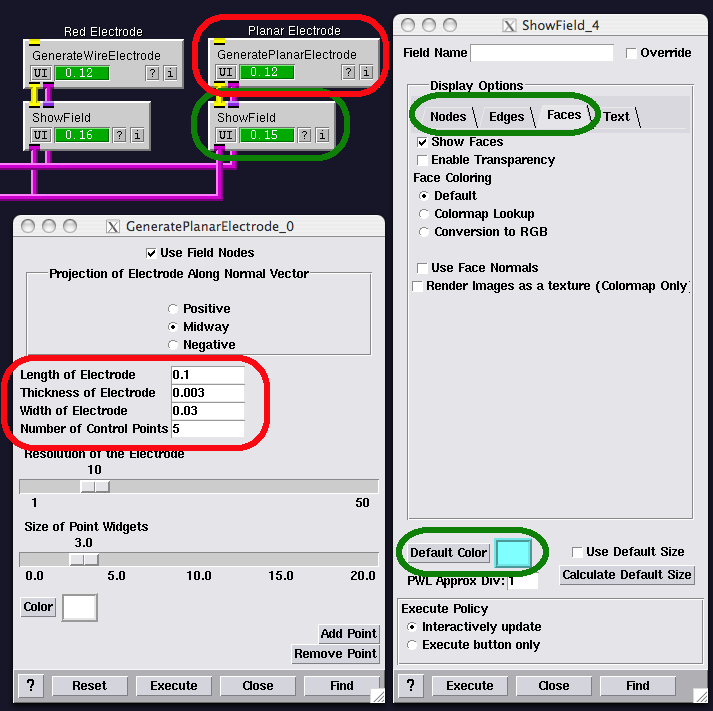
\includegraphics{DefibrillationTutorial_figures/place_electrodes_network_6.png}}
\caption{Addition of a planar electrode.}\label{fig:p_e_network_6}
\end{figure}

\begin{figure}
\scalebox{0.3}{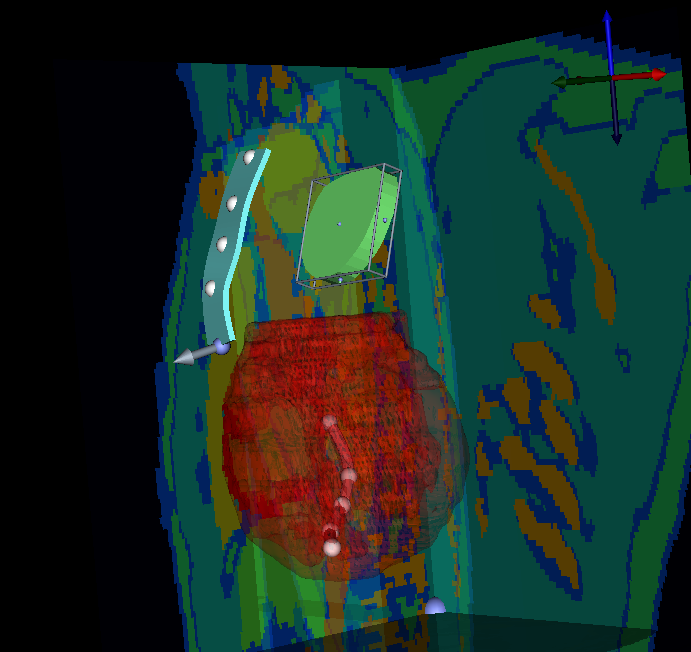
\includegraphics{DefibrillationTutorial_figures/place_electrodes_results_6}}
\caption{Placement of the planar electrode.}\label{fig:p_e_results_6}
\end{figure}

\section{Writing Electrodes to a Bundle}\label{sec:write_bundle}

One feature of SCIRun is the ability to ``bundle'' various fields
together. We will take advantage of that feature when writing the
electrode fields to a file. Add a {\bf InsertFieldsIntoBundle} module
into the network and connect the yellow output of the can electrode's
{\bf EditMeshBoundingBox} module to the first input. Connect the
outputs of the two {\bf GenerateElectrode} modules to the second and
third inputs of
{\bf InsertFieldsIntoBundle}. Open the user interface and click on the
``Field 1'' tab. In the ``Name'' textbox, type a descriptive name for
the first field, such as {\tt CAN ELECTRODE}. Click on the ``Field 2''
tab and provide a name, such as {\tt WIRE ELECTRODE}. Click on the
``Field 3'' tab and provide a name, such as {\tt PLANAR ELECTRODE}.

Next, connect the orange output of {\bf InsertFieldsIntoBundle} to a
new {\bf WriteBundle} module. Open the user interface, browse for a
directory, and type a name for the electrode field bundle save
file. Executing that module will cause the file to be written. Figure
\ref{fig:p_e_network_7} shows the complete network.

\begin{figure}
\scalebox{0.35}{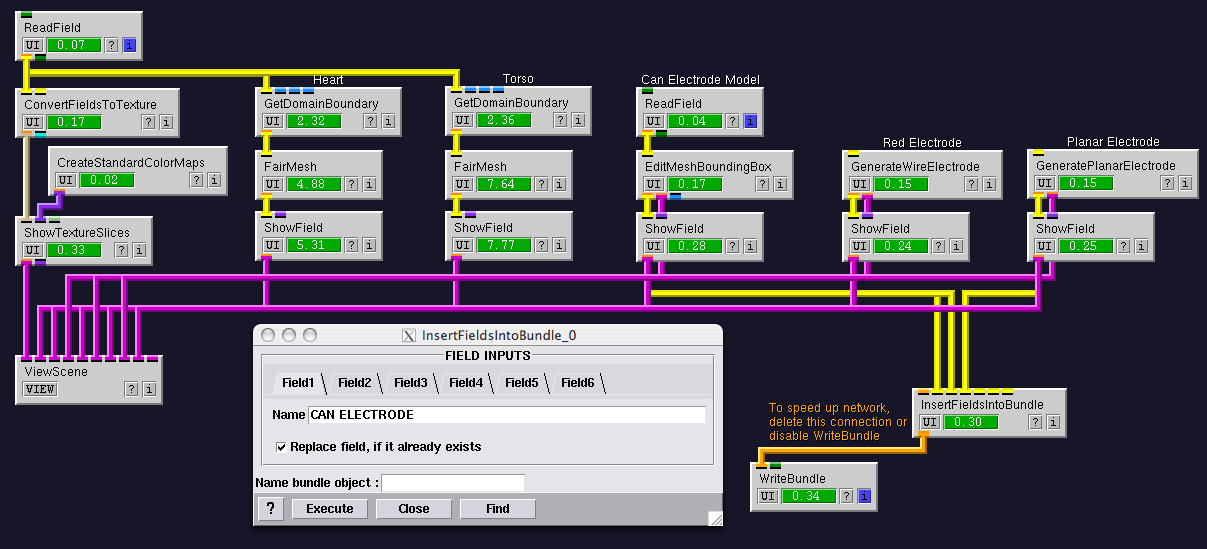
\includegraphics{DefibrillationTutorial_figures/place_electrodes_network_7.png}}
\caption{Complete network for generating and placing
electrodes.}\label{fig:p_e_network_7}
\end{figure}

Note that if the {\bf WriteBundle} module is connected and enabled,
each time the network is run, the file will be overwritten. Thus, if
you move one of the electrode in the view window, the old file will be
automatically overwritten with the new file. To keep this from
happening, disconnect the {\bf WriteBundle} module until you are ready
to write the file, or right click on the module and select ``Disable''
from the dropdown menu.

\chapter{Finite Element Simulation on a Torso}

In the previous chapter, we created a network which allows the
placement of various electrodes within a torso. The result of that
network was a SCIRun bundle being written to a file, consisting of
three fields: a can electrode, a wire electrode, and a planar
electrode. In this chapter, we will read the torso and the electrodes
back in, assign known conductivities to various materials in the torso
segmentation, assign known potentials to two of the electrodes, allow
the third electrode to be a floating lead, create a finite element
mesh, refine that mesh near the electrodes, and solve the electric
field problem.

\section{Building and Viewing the Finite Element Mesh}

To simplify processing and reduce runtimes, we will create a smaller
Hexahedral Mesh on which the finite element simulation will be run. To
do this, start a new network and insert a {\bf ReadField} module. Open
the module, select ``SCIRun Field File (*.fld)'' in the ``Fields of
type'' dropdown box, browse for and select the {\tt
segmentation\_si.fld} file. Connect the output to a {\bf CreateLatVol}
module. In {\bf CreateLatVol}, set the ``X Size'', ``Y Size'', and ``Z
Size'' text fields to {\tt 50}, {\tt 50}, and {\tt 75}. Insert a {\bf
MapFieldDataOntoElems} module into the network, connecting the output
of {\bf ReadField} to the first input and the output of {\bf
CreateLatVol} to the third input. This will map the data values in the
segmentation onto the nodes of the hex mesh. Open the {\bf
MapFieldDataOntoElems} module and select ``mostcommon'' in the
``SampleMethodPerElement'' dropdown box. This will ensure the values
on the nodes will be one of the segmentation values and not an
interpolated value. Figure \ref{fig:defib_fem_nw_01} shows this new
network.

\begin{figure}
\scalebox{0.4}{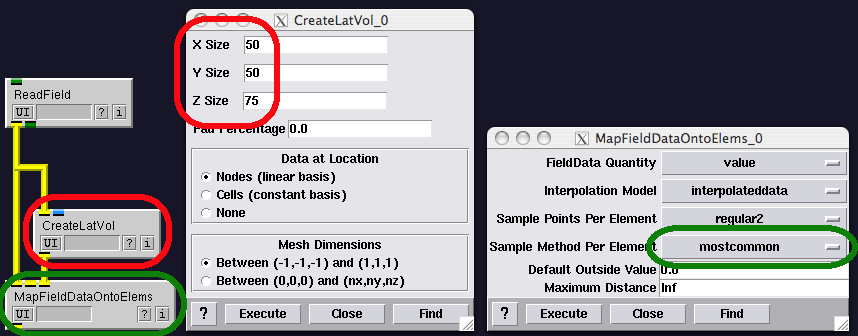
\includegraphics{DefibrillationTutorial_figures/defib_fem_nw_01.png}}
\caption{Beginnings of the defibrillation finite element simulation
network.}\label{fig:defib_fem_nw_01}
\end{figure}

To visualize the segmentation, first we will clip the data outside the
actual torso (outside data has a value of {\tt 0}) by connecting a
{\bf ClipFieldByFunction} module to the output of {\bf
MapFieldDataOntoElems}. Open the user interface and set the expression
to {\tt RESULT=DATA>0;}. Next, connect the output of {\bf
MapFieldDataOntoElems} to the following module chain: {\bf
GetFieldBoudnary}, {\bf FairMesh}, {\bf ShowField}, and {\bf
ViewScene}. As we did in the entire last chapter, open the {\bf
ShowField} module and disable rendering of the nodes and edges. Figure
\ref{fig:defib_fem_nw_r_02} shows this new network and the resulting
visualization.

\begin{figure}
\scalebox{0.4}{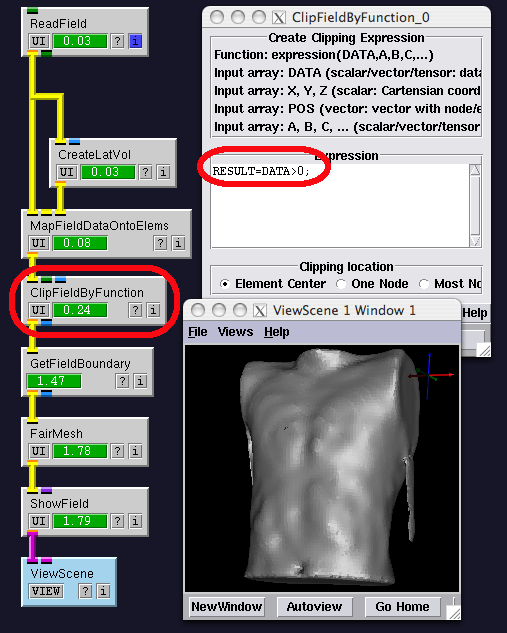
\includegraphics{DefibrillationTutorial_figures/defib_fem_nw_r_02.png}}
\caption{Viewing the finite element torso
mesh.}\label{fig:defib_fem_nw_r_02}
\end{figure}

\section{Completing an Initial Two-Electrode Simulation}

Now that our simulation mesh has been created, we need to build our
finite element matrix, add our known electric potentials in the
locations of the electrodes, and solve the finite element linear
system. We will start by specifying the conductivities of various
materials in the segmentation. To do so, insert a {\bf CreateMatrix}
module into the network. Open the user interface and set the number of
rows to {\tt 12} and the number of columns to {\tt 1} by typing these
values into the text boxes at the top. A matrix with 12 entries (0
through 11) will appear. Table \ref{tbl:conductivities} lists the
conductivities used in this simulation. Populate the matrix with
these, or modified values.

\begin{table}[h]
\begin{tabular}{|l|l|l|}
\hline
{\bf Material} & {\bf Seg. Indx} & {\bf Conductivity (S/m)} \\
\hline \hline
Background & 0 & 0.0\\ \hline
Connective Tissue & 1 & 0.22\\ \hline
Bowel Gas & 2 & 0.002\\ \hline
Muscle & 3 & 0.25\\ \hline
Fat & 4 & 0.05\\ \hline
Kidney & 5 & 0.15\\ \hline
Liver & 6 & 0.07\\ \hline
Lung & 7 & 0.007\\ \hline
Bone & 8 & 0.006\\ \hline
Blood & 9 & 0.7\\ \hline
Heart-Atria & 10 & 0.3\\ \hline
Heart-Ventricles & 11 & 0.3\\ \hline
\end{tabular}
\caption{Conductivity values used in this simulation.} \label{tbl:conductivities}
\end{table}

Connect the yellow output of {\bf ClipFieldByFunction} to the input of
a {\bf ConvertIndicesToFieldData} module. Connect the output of {\bf
CreateMatrix} to the second input. Connect the output of {\bf
ConvertIndicesToFieldData} to a {\bf BuildFEMatrix} module. The
network should look similar to Figure \ref{fig:defib_fem_nw_03}.

\begin{figure}
\scalebox{0.4}{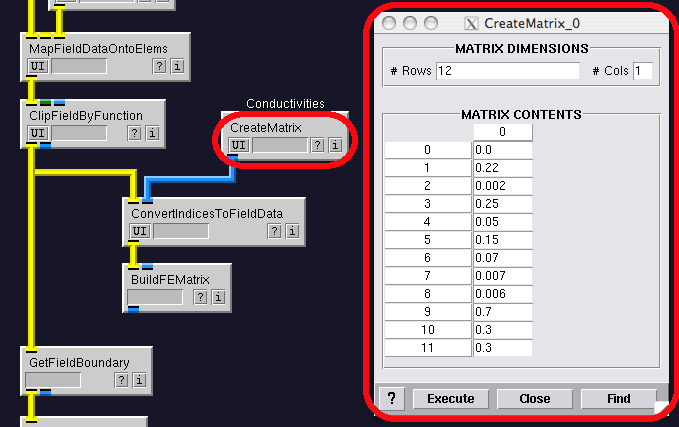
\includegraphics{DefibrillationTutorial_figures/defib_fem_nw_03.png}}
\caption{Network now incorporating conductivities and the finite
element matrix.}\label{fig:defib_fem_nw_03}
\end{figure}

Next, the electrodes need to be incorporated into the
simulation. Insert a {\bf ReadBundle} module into the network. Open
and select the electrode bundle written previously to a file in
Section \ref{sec:write_bundle}. Connect the output of {\bf ReadBundle}
to a {\bf GetFieldsFromBundle} module. For the user interface of {\bf
GetFieldsFromBundle} to work correctly, the {\bf ReadBundle} module
needs to first be executed. Right click on {\bf ReadBundle} and select
``Execute'' from the pop-up menu. Now, open the {\bf
GetFieldsFromBundle} user interface. We will need to specify which
fields in the bundle will correspond to the output ports on the
module. Make sure the ``Field1'' tab is selected, and click on {\tt
CAN ELECTRODE} in the selection list (or whatever the can electrode
field was named previously. Open the ``Field2'' tab and select {\tt
WIRE ELECTRODE}. Open the ``Field3'' and select {\tt PLATE
ELECTRODE}. This will associate the can, wire, and plate electrodes
with the first, second, and third yellow output ports. Figure
\ref{fig:defib_fem_nw_04} shows the addition of these modules to the
network.

\begin{figure}
\scalebox{0.4}{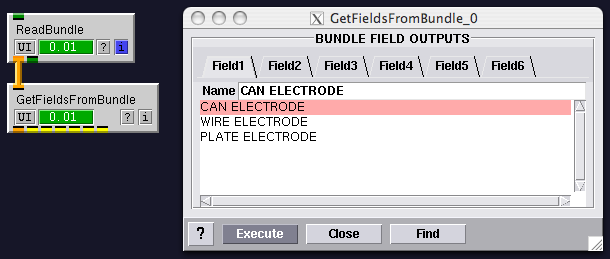
\includegraphics{DefibrillationTutorial_figures/defib_fem_nw_04.png}}
\caption{Reading in the electrode configuration
bundle.}\label{fig:defib_fem_nw_04}
\end{figure}

We will use a slightly different technique for associating known
potentials to the electrodes than we did with the box simulation. To
start, connect the first and second yellow outputs of {\bf
GetFieldsFromBundle} to separate {\bf CreateFieldData}
modules. Connect those modules to a {\bf JoinFields} module. In the
first {\bf CreateFieldData} module, set the function to {\tt RESULT =
1;}. In the second, set the function to {\tt RESULT = 2;}. These
network additions are shown in Figure \ref{fig:defib_fem_nw_05}.

\begin{figure}
\scalebox{0.4}{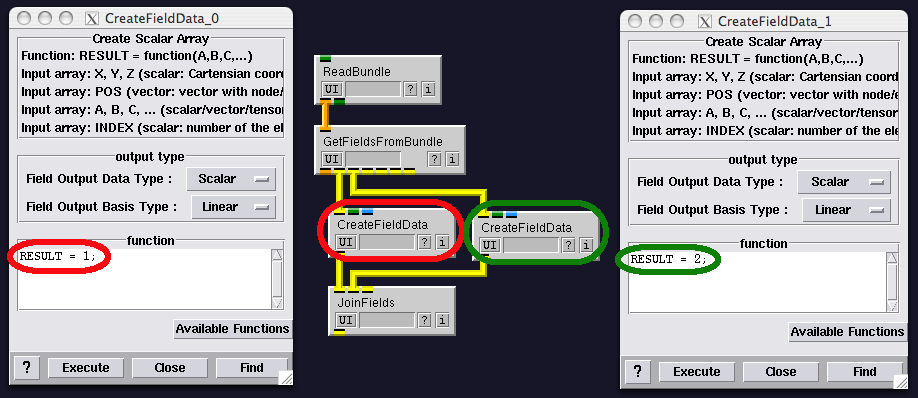
\includegraphics{DefibrillationTutorial_figures/defib_fem_nw_05.png}}
\caption{Specifying field labelings for the two electrode
fields.}\label{fig:defib_fem_nw_05}
\end{figure}

Next, we will map these indices onto our mesh, giving us a mesh with
values of {\tt 1} where at the can electrode, {\tt 2} at the wire
electrode, and {\tt 0} everywhere else. We accomplish this by
connecting the {\bf JoinFields} module to the first input of a {\bf
MapFieldDataOntoNodes} module. Connect the output of {\bf
ClipFieldByFunction} to the third input of the new {\bf
MapFieldDataOntoNodes} module. Similar to how we mapped conductivities
onto the mesh, we will map the known potentials onto the mesh using a
new {\bf ConvertIndicesToFieldData}, which receives its input from the
{\bf MapFieldDataOntoNodes} module and a new {\bf CreateMatrix}
module. Open the {\bf CreateMatrix} user interface, and set the number
of rows and number of columns to {\tt 4} and {\tt 1}.

Remember from the box tutorial that a value of NaN in our ``known
values'' vector signifies an unknown value. Therefore, we set the
first entry of our matrix to a value of {\tt nan}. The next two
entries represent the potentials of the two electrodes. We will set
these to {\tt 450} and {\tt 0} for this simulation. Finally, for
reasons that will become clear once we add a floating electrode, set
the fourth entry to {\tt nan}. The current state of the network is
shown in Figure \ref{fig:defib_fem_nw_06}.

\begin{figure}
\scalebox{0.4}{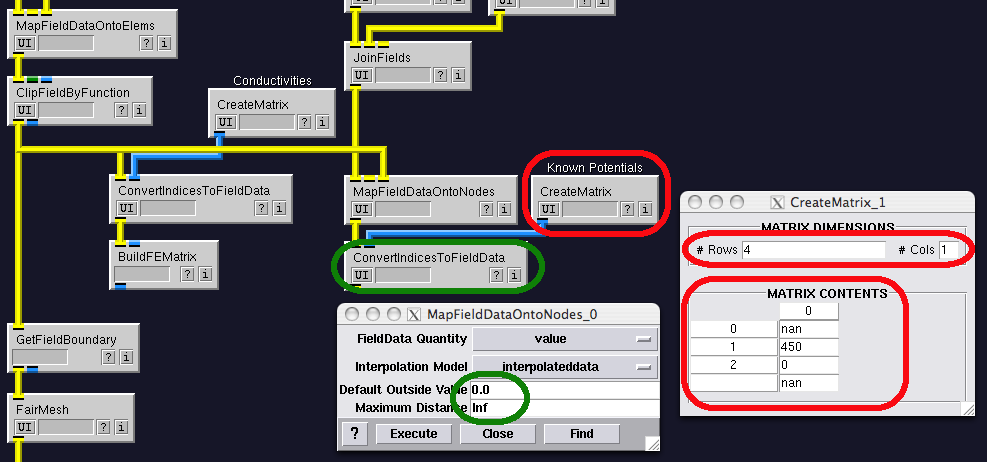
\includegraphics{DefibrillationTutorial_figures/defib_fem_nw_06.png}}
\caption{Associating known potential values with the two
electrodes.}\label{fig:defib_fem_nw_06}
\end{figure}

The values on the mesh now represent the ``known'' values of our
solution. All that remains to complete our first simulation is to get
a vector of these known values and add them as known values to our
linear system. To do this, connect the {\bf ConvertIndicesToFieldData}
module to a {\bf GetFieldData} module. Add a {\bf
AddKnownsToLinearSystem} module with the first input coming from {\bf
BuildFEMatrix} and the third input coming from the {\bf GetFieldData}
module. Connect the two outputs of {\bf AddKnownsToLinearSystem} to
the two inputs of a {\bf SolveLinearSystem} module. These
modifications are shown in Figure \ref{fig:defib_fem_nw_07}.

\begin{figure}
\scalebox{0.4}{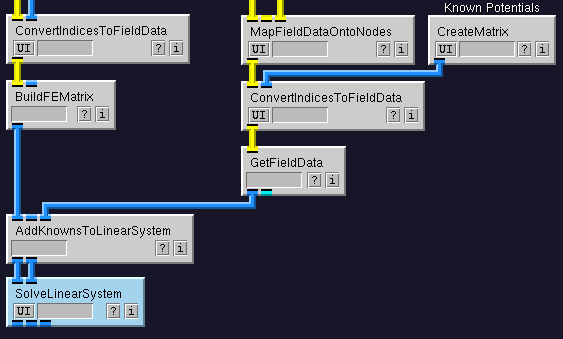
\includegraphics{DefibrillationTutorial_figures/defib_fem_nw_07.png}}
\caption{Solving the linear system.}\label{fig:defib_fem_nw_07}
\end{figure}

To visualize the results at this point, insert a {\bf SetFieldData}
module between the current {\bf ClipFieldByFunction} and {\bf
GetFieldBoundary} modules. This requires deleting the previous
connection, adding the module, and connecting the three modules
together. We will add a standard color map by adding a {\bf
CreateStandardColorMaps} module connected to a {\bf RescaleColorMap}
module. The second input of the {\bf RescaleColorMap} module comes
from the output of the {\bf SetFieldData} module. The output of {\bf
RescaleColorMap} is used as the second input for the {\bf ShowField}
module. Open the {\bf ShowField} module and make sure the ``Face
Coloring'' on the ``Faces'' tab is now set to ``Colormap
Lookup''. These changes and the resulting visualization are shown in
Figure \ref{fig:defib_fem_nw_r_08}.

\begin{figure}
\scalebox{0.4}{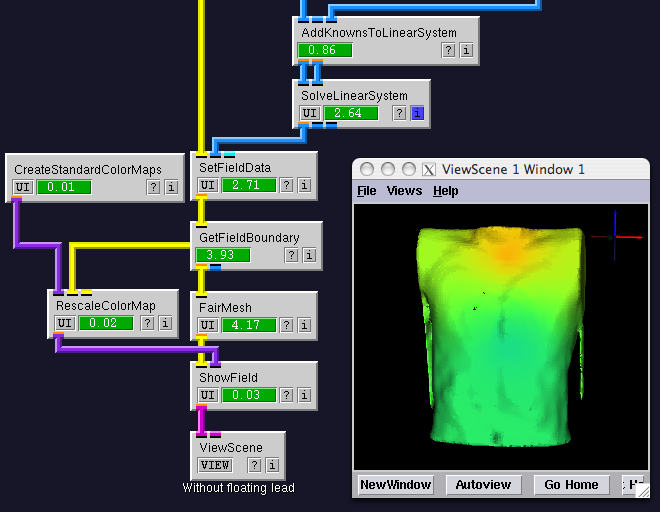
\includegraphics{DefibrillationTutorial_figures/defib_fem_nw_r_08.png}}
\caption{Initial simulation results for the two electrode
problem.}\label{fig:defib_fem_nw_r_08}
\end{figure}

\section{Refining the Mesh}

Depending on the resolution of the mesh generated in the {\bf
CreateLatVol} module, and depending on the size of the electrodes used
in the simulation, the electrodes may be much smaller than can be
resolved on our simulation mesh. Our first modification to the
simulation in the previous section is to perform automatic refining of
the mesh close to the electrodes.

Start by deleting the connection between {\bf CreateLatVol} and {\bf
MapFieldDataOntoElems}. Connect the output of {\bf CreateLatVol} to a
{\bf CalculateDistanceToField} module. Connect the output of {\bf
JoinFields} to the second input. Next, we will map this data back onto
the the simulation mesh by connecting the output of {\bf
CalculateDistanceToField} to a {\bf MapFieldDataOntoElems} module. The
third input of the new {\bf MapFieldDataOntoElems} comes directly from
{\bf CreateLatVol}. This distance information is now used to drive the
refinement of the mesh. Elements with distances close to the
electrodes will be refined while elements further away will be left as
is. This refinement is accomplished by connecting the output of {\bf
MapFieldDataOntoElems} to a {\bf RefineMesh} module. Lastly, connect
the output of {\bf RefineMesh} to the third input of our original {\bf
MapFieldDataOntoElems} module (which was partially disconnected at the
beginning of this procedure).

The user interface settings are as follows: Open the {\bf
CalculateDistanceToField} module and check the ``Truncate distance
larger than:'' checkbox. Insert a value of {\tt 0.02} in the text
box. Open the newest {\bf MapFieldDataOntoElems} module, and select
``max'' from the ``Sample Method Per Element'' dropdown menu. Open the
{\bf RefineMesh} module, select the ``Do not refine nodes/elements
with values greater than isovalue'' radio button, and enter an
IsoValue of {\tt 0.02} in the text box. Figure
\ref{fig:defib_fem_nw_09} shows these additions to the network while
Figure \ref{fig:defib_fem_r_09} shows the simulation results.

\begin{figure}
\scalebox{0.4}{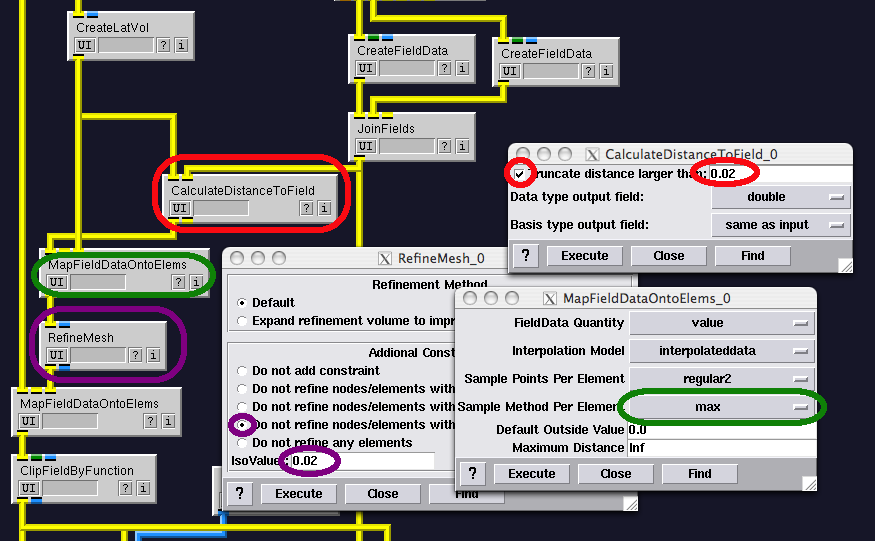
\includegraphics{DefibrillationTutorial_figures/defib_fem_nw_09.png}}
\caption{Adding functionality to refine the mesh near the
electrodes.}\label{fig:defib_fem_nw_09}
\end{figure}

\begin{figure}
\scalebox{0.4}{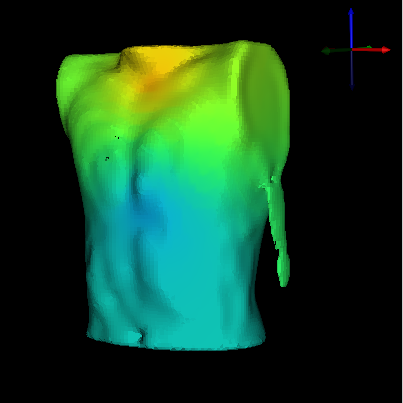
\includegraphics{DefibrillationTutorial_figures/defib_fem_r_09.png}}
\caption{Simulation results after mesh
refinement.}\label{fig:defib_fem_r_09}
\end{figure}

\section{Adding a Floating Lead}

As in the box simulation, we may wish to add a floating lead, or a
conductor, to our simulation. We will use the plate electrode saved in
our input bundle as this floating lead. The first step is to connect
the third yellow output from the {\bf GetFieldsFromBundle} a
{\bf CreateFieldData} module (with equation set to {\tt
RESULT = 3;}), and connect that output to the {\bf JoinFields}
module. Remember that our second {\bf CreateMatrix} containing known
potentials contains and extra value of {\tt nan} for the fourth
entry. Therefore, the plate electrode will still be considered an
unknown value. The remainder of the addition of the floating electrode
is very similar to the box example in Chapter \ref{sec:cube}.

Insert a new {\bf CalculateInsideWhichField} module, with the first
input coming from the {\bf ClipFieldByFunction} module, and the second
input coming from the {\bf CreateFieldData} module associated with the
plate electrode. Open the user interface and set the ``Default outside
value'' to {\tt nan}. Set the ``Datatype of destination field'' to
``float'' and set the ``Output data location'' to ``node''. Connect
the output to a {\bf GetFieldData} module. The current state of the
network is shown in Figure \ref{fig:defib_fem_nw_10}.

\begin{figure}
\scalebox{0.35}{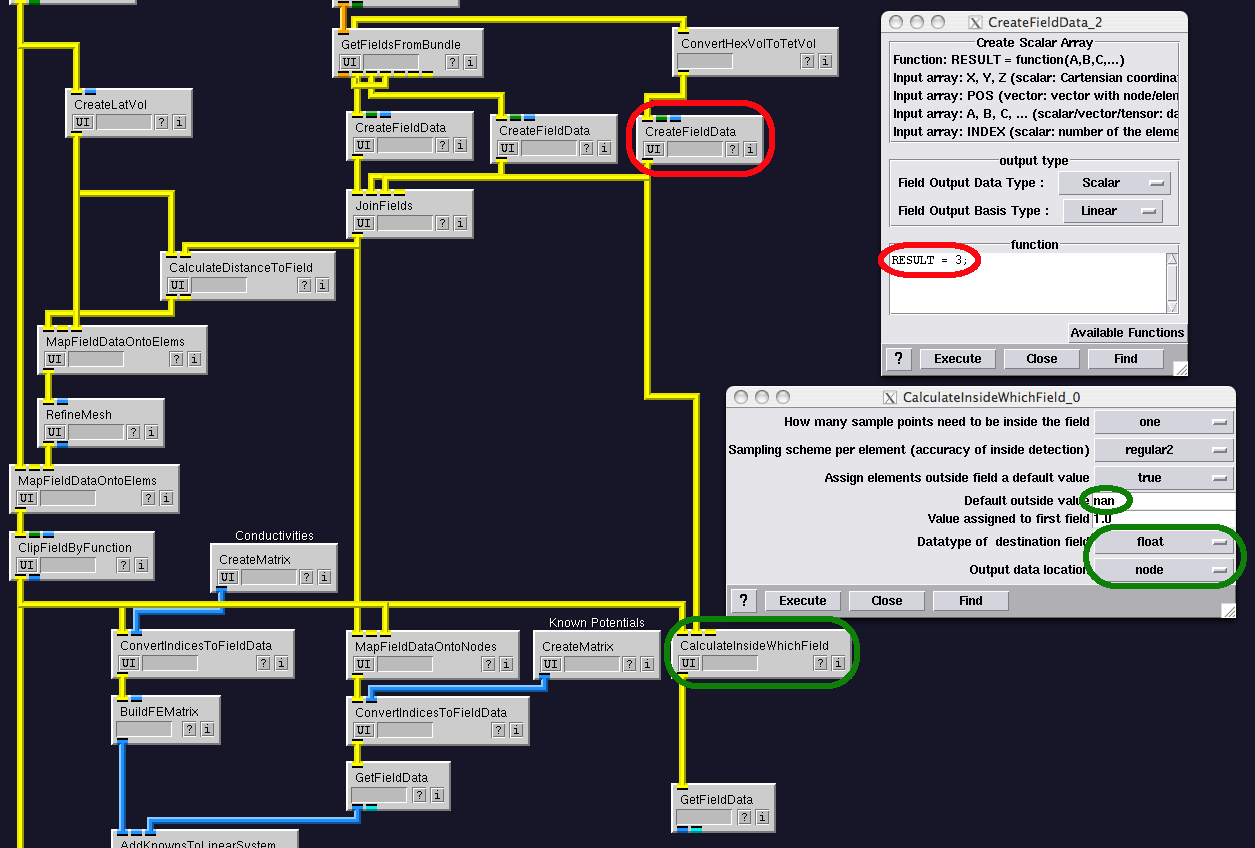
\includegraphics{DefibrillationTutorial_figures/defib_fem_nw_10.png}}
\caption{Adding a floating electrode to the
simulation.}\label{fig:defib_fem_nw_10}
\end{figure}

We will now create a second simulation pathway instead of modifying
the first simulation which will help show the differences between the
simulation with and without the floating electrode. Connect the two
outputs of {\bf AddKnownsToLinearSystem} to the first two inputs of
{\bf AddLinkedNodesToLinearSystem}. The third input comes from the
latest {\bf GetFieldData} module. Connect the first two outputs of
{\bf AddLinkedNodesToLinearSystem} to a {\bf SolveLinearSystem}
module. Connect the third output of {\bf AddLinkedNodesToLinearSystem}
to the first input of a {\bf EvaluateLinAlgBinary} module. The second
input of the {\bf EvaluateLinAlgBinary} comes from the first output of
{\bf SolveLinearSystem}. Create a new {\bf SetFieldData} module, the
first input coming from the {\bf ClipFieldByFunction} module, and the
second input coming from the {\bf EvaluateLinAlgBinary}
module. Duplicate the remainder of the first simulation pathway after
the {\bf SetFieldData} module (starting with the {\bf
GetFieldBoundary} module. These modifications are shown in Figure
\ref{fig:defib_fem_nw_11} with the simulation results shown in Figure
\ref{fig:defib_fem_r_11}.

\begin{figure}
\scalebox{0.4}{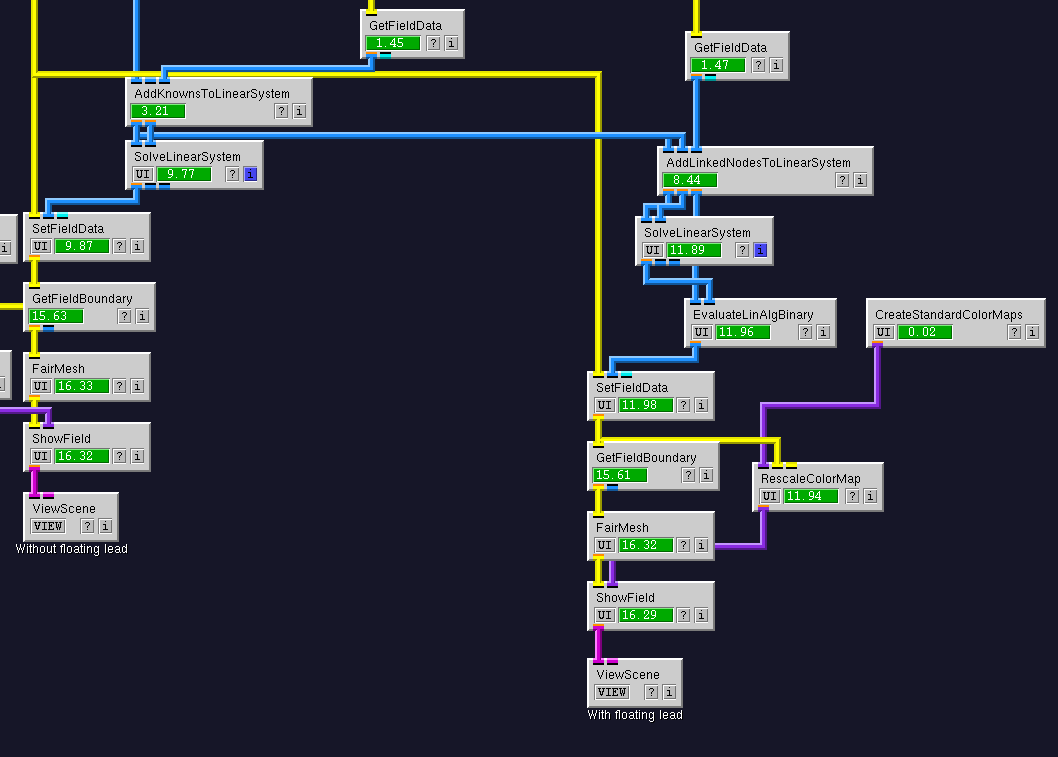
\includegraphics{DefibrillationTutorial_figures/defib_fem_nw_11.png}}
\caption{Second simulation pathway including a floating
electrode.}\label{fig:defib_fem_nw_11}
\end{figure}

\begin{figure}
\scalebox{0.4}{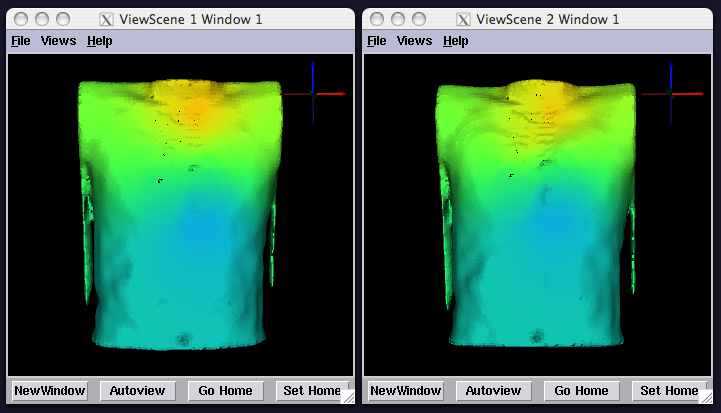
\includegraphics{DefibrillationTutorial_figures/defib_fem_r_11.png}}
\caption{Results both with (right) and without (left) a floating
electrode.}\label{fig:defib_fem_r_11}
\end{figure}

The differences between the two simulations in Figure
\ref{fig:defib_fem_r_11} are admittedly difficult to discern. Our last
step, therefore, will be to create a visualization of the differences
between these two simulations. Connect the outputs of the {\bf
SolveLinearSystem} (without the floating lead) and the {\bf
EvaluateLinAlgBinary} (with the floating lead) to another {\bf
EvaluateLinAlgBinary} module. Open the user interface and select the
``Function'' radio button, typing {\tt x - y} into the ``Specify
function'' text box. Create yet another {\bf SetFieldData} module,
with the first input again coming from the {\bf ClipFieldByFunction}
module and the second input coming from the newest {\bf
EvaluateLinAlgBinary} module. Duplicate the remaining visualization
pipeline. This time, however, select a color map which deemphasizes
values near zero. The ``BP Seismic'' colormap will do this. Figure
\ref{fig:defib_fem_nw_12} shows the final additions to the network
while Figure \ref{fig:defib_fem_r_12} shows the differences between
the two simulations.

\begin{figure}
\scalebox{0.4}{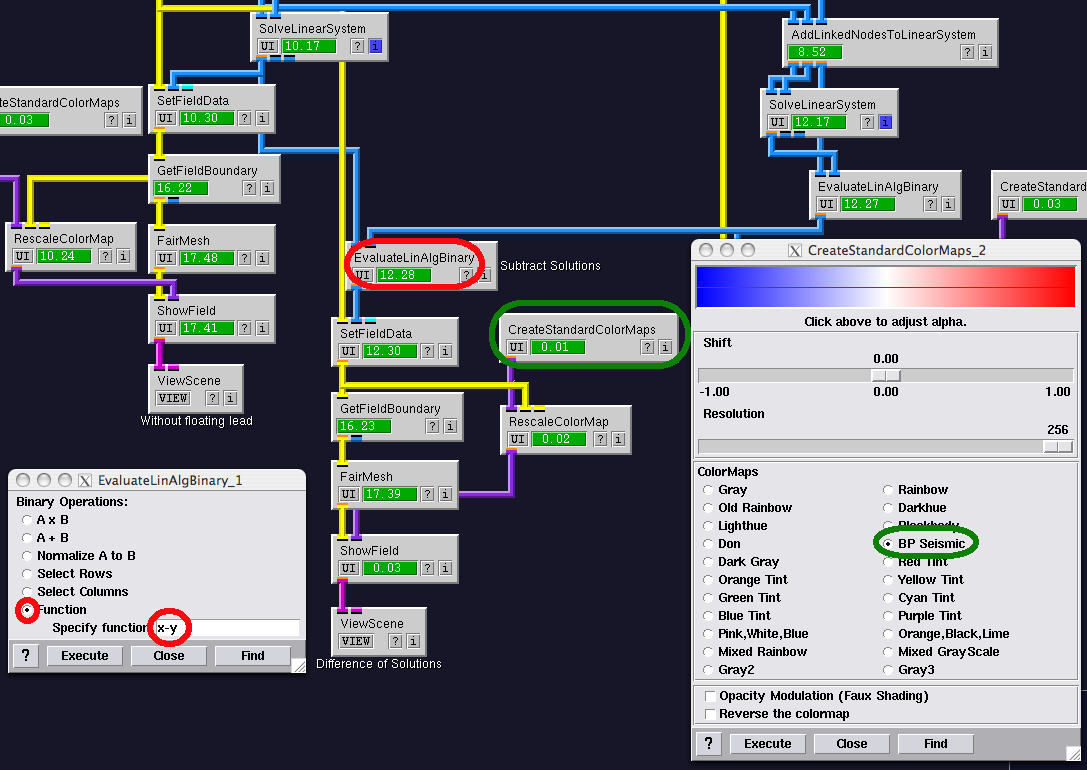
\includegraphics{DefibrillationTutorial_figures/defib_fem_nw_12.png}}
\caption{Adding a visualization pipeline to show differences between
the solutions with and without a floating
lead.}\label{fig:defib_fem_nw_12}
\end{figure}

\begin{figure}
\scalebox{0.4}{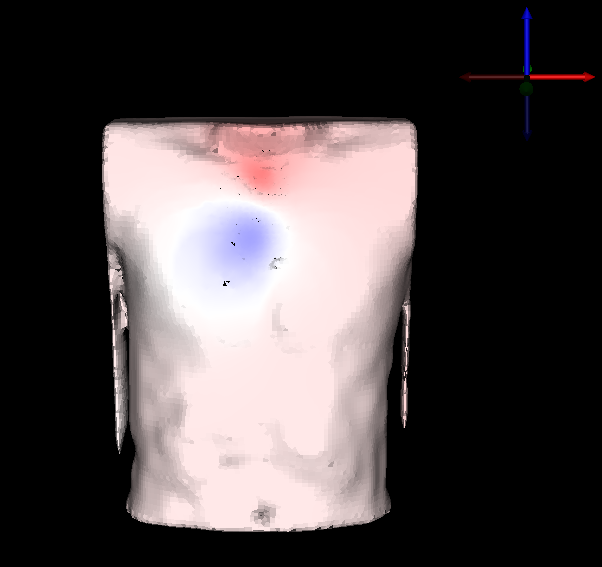
\includegraphics{DefibrillationTutorial_figures/defib_fem_r_12.png}}
\caption{Results showing differences between two solutions--one with
and one without a floating lead.}\label{fig:defib_fem_r_12}
\end{figure}

\end{document}